\documentclass[12pt,a4paper]{report}

% ================= GCTU FACULTY OF ENGINEERING MARGINS =================
% Top: 2.5 cm; Bottom: 2.5 cm; Left: 4.0 cm (for binding); Right: 2.5 cm
\usepackage[top=2.5cm, bottom=2.5cm, left=4.0cm, right=2.5cm]{geometry}

% ================= TYPOGRAPHY & SPACING =================
\usepackage{setspace}
\onehalfspacing % 1.5 line spacing per handbook

% Paragraphing: First line must NOT be indented; paragraphs line-spaced
\setlength{\parindent}{0pt}
\setlength{\parskip}{1em}

% ================= CORE PACKAGES =================
\usepackage{graphicx}
\graphicspath{{figures/}{../docs_and_figures/}{../maps/}{../test_pics/}}
\usepackage{amsmath,amssymb,amsfonts}
\usepackage{booktabs,array,ragged2e,longtable,pdflscape,float}
\usepackage{url}
\usepackage{cite}
\usepackage{xcolor}
\usepackage[hidelinks]{hyperref}

% Table caption above, figure caption below (Handbook Section 2.3)
\usepackage[tableposition=top,figureposition=bottom]{caption}

\begin{document}

% ================= MAIN BODY CHAPTERS =================
\pagenumbering{arabic}
\setcounter{page}{1}

\chapter{Introduction}

\section{Background of the Study}
Robotics engineering has transitioned rapidly from isolated industrial work-cells toward dynamic, human-centered environments where machines and humans share physical workspaces. In these collaborative settings, autonomous mobile robots are required to operate intelligently alongside human personnel rather than merely executing rigid, pre-programmed trajectories in segregated areas. This operational shift has established Human-Robot Interaction (HRI) as a foundational discipline in modern robotics, requiring machines to interpret human social cues and intentions with high operational reliability. For an autonomous mobile robot to function safely and intuitively in shared spaces, it must recognize, interpret, and respond to human behavior in a manner that is predictable, natural, and immediate.

A primary communication channel in human-to-human collaboration is the use of natural hand gestures and body movement cues. Although modern computer vision algorithms have made optical gesture recognition increasingly practical, conventional deep learning implementations typically rely on cloud infrastructure or power-intensive Graphics Processing Units (GPUs) \cite{mahmud2022}. This reliance introduces severe communication latencies and vulnerability to network interruptions, rendering remote processing impractical for time-critical robotic safety applications \cite{tsitos2022}. Furthermore, a mobile robotic system cannot operate effectively by merely classifying gestures in isolation; it must maintain active spatial awareness of its surrounding environment to execute navigational directives safely. This study addresses these interconnected challenges by engineering and physically deploying a unified, vision-based intention recognition and autonomous navigation pipeline operating strictly on an embedded edge computing platform.

\section{Problem Statement}
Despite significant advancements in collaborative robotics, achieving seamless, responsive, and robust human-robot collaboration on low-cost, resource-constrained hardware remains an unresolved engineering bottleneck. Most industrial and commercial service robots still depend on rigid control modalities, such as physical teach pendants, capacitive touchscreens, or acoustic voice commands. These conventional interfaces frequently prove ineffective in noisy industrial manufacturing facilities or sterile healthcare environments where physical contact must be strictly avoided.

Moreover, existing vision-based intention recognition frameworks exhibit three critical technological limitations when transitioned to real-world embedded deployment:
\begin{enumerate}
    \item \textbf{High-Power Hardware and Cloud Dependency:} Many contemporary vision-based gesture architectures rely heavily on high-end desktop GPUs or offboard cloud computing services for inference \cite{mahmud2022}. In mobile robotics, reliance on offboard processing introduces unpredictable network latency, consumes excessive power, and introduces single-point network failure risks that violate real-time safety thresholds \cite{tsitos2022}.
    \item \textbf{Spatial Coordinate Domain Shift Across Distances:} Standard machine learning classifiers frequently evaluate raw anatomical pixel coordinates extracted from image frames. Because absolute landmark coordinates vary drastically as an operator moves closer to or farther from the camera, conventional models suffer severe classification degradation under real-world operational distance variations.
    \item \textbf{Ungrounded and Spatial-Blind Command Execution:} Existing gesture-controlled mobile robots predominantly execute motor commands blindly without contextual awareness of their physical surroundings. Translating recognized gestures into motor velocities without continuous laser-based environment mapping and obstacle verification presents immediate collision hazards in populated indoor workspaces.
\end{enumerate}

To overcome these engineering limitations, there is a distinct requirement for a lightweight, edge-deployable framework that tightly couples real-time intention recognition with spatial mapping within a unified, standardized robotic middleware.

\section{Objectives of the Study}

\subsection{General Objective}
The general objective of this research is to design, implement, and empirically evaluate an edge-deployed, real-time human intention recognition and navigation system that integrates scale-invariant hand gesture classification, temporal motion prediction, and spatial mapping into a unified ROS2 middleware pipeline on an autonomous mobile robot.

\subsection{Specific Objectives}
To achieve this general objective, the following specific objectives were established:
\begin{enumerate}
    \item To design and implement an edge-optimized computer vision pipeline utilizing spatial zone filtering, anatomical hand landmark tracking, and a Multilayer Perceptron (MLP) classifier trained on nineteen engineered, scale-invariant geometric hand features.
    \item To construct, balance, and validate a custom 6,000-sample gesture dataset captured directly through the onboard monocular camera to eliminate sensor domain shift across six distinct operational commands.
    \item To develop a sequential motion prediction model utilizing a Long Short-Term Memory (LSTM) recurrent neural network to forecast short-horizon operator movement trajectories from continuous body pose landmarks.
    \item To implement a centralized, deterministic decision-making node (\texttt{brain\_node}) featuring temporal majority-vote confirmation, active subject-locking, and proportional visual servoing within a multi-node ROS2 Humble software architecture.
    \item To configure and physically validate Simultaneous Localization and Mapping (SLAM) and autonomous navigation stacks (Nav2) on the mobile platform to support safe, spatially aware trajectory execution.
    \item To quantitatively evaluate system performance through classification accuracy, confusion matrix analysis, component latency budgets, and real-time hardware throughput measurements on an embedded edge processor.
\end{enumerate}

\subsection{Engineering Research Questions}
In alignment with Faculty of Engineering standards, this study formulates four core Engineering Research Questions (ERQs) to evaluate the technical feasibility, mathematical invariance, multi-user robustness, and safety compliance of the deployed system:
\begin{enumerate}
    \item \textbf{ERQ 1 (Edge Feasibility and Latency Budget):} Can a multi-stage visual perception pipeline—incorporating person detection, twenty-one-point hand landmark extraction, and geometric feature computation—execute natively on a low-cost, low-power edge processor (Raspberry Pi 5) without GPU acceleration while maintaining an end-to-end processing cycle below the 150~ms human-interaction latency threshold?
    \item \textbf{ERQ 2 (Mathematical Feature Invariance):} To what extent does converting raw anatomical landmark coordinates into scale- and distance-invariant geometric features (joint curl angles and palm-normalized Euclidean distances) eliminate spatial distortion and improve gesture classification accuracy across varying operator distances compared to unnormalized coordinate baselines?
    \item \textbf{ERQ 3 (Multi-Person Workspace Disambiguation):} How effectively can a central geometric spatial-zone filter coupled with rolling majority-vote temporal buffering isolate and maintain an active control lock on a primary operator in a shared workspace, preventing unintended command execution from background bystanders?
    \item \textbf{ERQ 4 (Intention-to-Action Coupling and Safety Verification):} Can discrete hand gesture commands and continuous kinematic motion trajectories be reliably integrated within ROS2 middleware to govern mobile robot velocity commands in full compliance with ISO 15066 collaborative robotic safety and reaction requirements?
\end{enumerate}

\section{Scope of the Study}
The operational scope of this research is bounded to the design, software integration, and physical deployment of a gesture-directed autonomous mobile robot operating within indoor environments. The testing environment is restricted to structured indoor settings with stable floor surfaces and standard ambient fluorescent illumination to ensure predictable sensor characteristics. To maintain deterministic control and prevent command ambiguity, the visual interaction vocabulary is restricted to six predefined static hand gestures (STOP, GO, LEFT, RIGHT, BACK, FOLLOW) and five discrete body motion states (Approaching, Moving Away, Moving Left, Moving Right, Stationary). 

Interaction is programmatically constrained to a single validated human operator at any given time, enforced through spatial-zone acceptance filtering and temporal lock scheduling. Furthermore, to address network vulnerability and communication latency constraints, the entire perception, intention interpretation, and motor control software stack operates strictly onboard the robot's local processor without any reliance on remote cloud servers or offboard computing clusters. Real-time operation is defined as the capability of the onboard architecture to sustain an end-to-end sensing-to-actuation cycle sufficient to maintain responsive, jitter-free interaction at human operating speeds.

\section{Significance of the Study}
The engineering significance of this study lies in demonstrating that complex, multi-modal human intention recognition can be successfully decoupled from power-hungry workstation GPUs and external cloud infrastructure. By deploying lightweight, mathematically engineered feature extractors directly onto embedded edge hardware, this research provides a scalable, cost-effective blueprint for autonomous mobile robots operating in resource-constrained settings.

From a practical perspective, an autonomous mobile robot capable of interpreting touchless gestures and body motion addresses critical requirements across several industrial and civil domains. In acoustically noisy manufacturing environments, optical gesture recognition provides an intuitive, reliable control alternative where acoustic voice recognition routinely fails. In sterile medical facilities and cleanrooms, touchless optical interaction prevents physical contamination and preserves strict hygiene protocols by eliminating contact with shared touchscreens. Academically, this study contributes an open, modular ROS2 architecture that combines explicit gesture classification with predictive motion tracking and laser-based spatial mapping. Ultimately, this work supports safer, more intuitive human-robot collaboration by ensuring predictable machine responses that adhere to international safety standards for collaborative robotic workspaces \cite{iso150662016}.

\section{Organization of the Study}
This project report is systematically structured into five cohesive chapters in accordance with the university project guidelines. 

Chapter One introduces the research background, defines the specific engineering bottlenecks, formulates the general and specific objectives alongside the core Engineering Research Questions, and delineates the project's scope and significance. Chapter Two presents a comprehensive review of related literature, examining theoretical foundations in Human-Robot Interaction, analyzing prior works in gesture classification and intention-aware navigation, and identifying the precise technological gaps addressed by this research. 

Chapter Three details the complete system design and methodology, encompassing physical hardware specifications, Docker-based containerized software deployment, geometric feature mathematics, LSTM path predictor training, and centralized state machine architecture. Chapter Four presents the empirical testing procedures, experimental results, classification confusion matrices, latency budgets, hardware throughput benchmarks, and comparative literature benchmarking. Finally, Chapter Five concludes the thesis by synthesizing the primary engineering findings, discussing physical implementation constraints, and proposing concrete recommendations for future industrial extensions.

\chapter{Literature Review}

\section*{2.0 Overview}
\addcontentsline{toc}{section}{2.0 Overview}
This chapter presents a critical review of relevant literature in human intention recognition, optical gesture analysis, and autonomous robot navigation in collaborative workspaces. Existing research establishes that autonomous mobile systems can recognize gestures, infer human motion trajectories, and adapt navigation behaviors to enhance interaction safety. However, a significant proportion of these systems operate under controlled laboratory conditions, depend on specialized high-power sensing hardware, or decouple intention recognition from mobile navigation. Consequently, this study builds directly upon existing theoretical and empirical frameworks by integrating vision-based human motion tracking and geometric hand gesture classification into an edge-deployed, mobile robotic platform operating in a mapped indoor environment.

\section{Theoretical Review}
This research is theoretically grounded in the principles of Human-Robot Interaction (HRI), human intention theory, geometric landmark kinematics, and spatial mobile robotics. Human intention theory posits that human goal-directed actions contain early predictive cues embedded within movement trajectories, forming the computational foundation for anticipatory robotic response systems. Within contemporary Human-Robot Interaction paradigms, collaborative mobile robots are required to move beyond purely reactive obstacle avoidance toward proactive, context-aware interaction within human-shared operational domains.

The theoretical formulation of gesture and motion recognition in this study is based on the premise that human hand anatomical configurations can be modeled geometrically and topologically from single-frame landmark distributions. Static gesture classification relies on the principle that instantaneous spatial arrangements of hand joints provide sufficient discriminative features to distinguish discrete operational commands within a fixed vocabulary. Conversely, human movement trajectory prediction inherently requires temporal context, as instantaneous positions cannot reveal directional intent or velocity. This distinction necessitates a sequential modeling approach—specifically Long Short-Term Memory (LSTM) recurrent neural networks—to capture temporal dependencies across consecutive pose observations over a sliding temporal window.

Spatial mapping and localization theory provides the mathematical framework for continuous autonomous navigation between human interaction events. Simultaneous Localization and Mapping (SLAM) constructs an occupancy-grid representation of the physical environment, while probabilistic Monte Carlo algorithms estimate the robot's coordinate pose relative to the global reference frame. Finally, multi-modal perceptual fusion theory demonstrates that combining explicit command channels (hand gestures) with implicit contextual cues (kinematic motion trajectories) mitigates command ambiguity and enhances operational robustness. Together, these theoretical frameworks provide the formal basis for developing a unified robotic system capable of recognizing, predicting, and responding to human intentions on physical hardware.

\section{Review of Related Works}

\subsection{Review One: Real-Time Intention Prediction via Upper-Limb Kinematics}

\subsubsection{Research Topic and Authors}
\textit{Real-time Feasibility of a Human Intention Method Evaluated Through a Competitive Human--Robot Reaching Game} (Tsitos et al., 2022) \cite{tsitos2022}.

\subsubsection{Objectives}
The primary objective of Tsitos et al. was to develop and evaluate an edge-feasible human intention prediction framework using a single RGB-D camera and the OpenPose skeletal tracking library. The authors aimed to integrate this predictive module into a standard ROS-based robotic control pipeline to govern arm trajectories in real time. Furthermore, the study investigated whether an industrial manipulator could react sufficiently early during competitive reaching tasks based on anticipatory kinematics rather than post-motion feedback.

\subsubsection{Methodology}
The authors implemented an experimental pipeline combining real-time human pose estimation with machine learning classification. An RGB-D camera captured upper-body human motion, from which OpenPose extracted 2D and 3D wrist joint coordinates during reaching movements. Raw spatial coordinates were digitally filtered to eliminate tracking jitter and segmented into distinct kinematic movement phases. Feature vectors were subsequently constructed from velocity and position profiles to train multiple classification models, including Support Vector Machines (SVM), Logistic Regression, Decision Trees, and Naive Bayes classifiers. The finalized predictive pipeline was interfaced directly into a ROS environment to control a 6-DOF Universal Robots UR3 manipulator during competitive reaching tasks.

\subsubsection{Strengths}
The investigation demonstrates that accurate intention prediction can be achieved using a streamlined, cost-effective setup comprising a single monocular depth sensor. By restricting the feature space to minimal wrist joint coordinates, the system sustained low-latency inference suitable for time-critical robotic interaction. The physical deployment on an industrial UR3 manipulator provided empirical validation on real hardware rather than simulated kinematics. Additionally, the experimental identification of a strict human reaction time threshold emphasized the critical role of processing latency in collaborative robotics.

\subsubsection{Limitations}
A primary limitation of the study is that the evaluation was confined to a static tabletop reaching game without mobile base movement. The human operator and the robotic arm did not share a contiguous mobile floor space, preventing the evaluation of spatial navigation or dynamic obstacle avoidance. Furthermore, the system relied exclusively on implicit reaching motion, offering no explicit gesture command channel through which the human could issue deliberate supervisory directives.

\subsubsection{Research Gap}
While Tsitos et al. demonstrated that kinematic intention prediction can operate within strict latency bounds, their architecture is restricted to a stationary manipulator arm. The robot and human never navigate a shared physical floor environment, and the human possesses no mechanism to command the robot through deliberate, explicit gestures. This leaves a distinct engineering gap between fast, stationary intention inference and its deployment onto an autonomous mobile platform capable of accepting both explicit gesture commands and navigating physical spaces.

\subsection{Review Two: 3D Skeletal Tracking and Adaptive Gesture Classification}

\subsubsection{Research Topic and Authors}
\textit{3D Gesture Recognition and Adaptation for Human--Robot Interaction} (Mahmud et al., 2022) \cite{mahmud2022}.

\subsubsection{Objectives}
The core objective of Mahmud et al. was to develop a three-dimensional hand gesture recognition and adaptation architecture capable of identifying both pointing and dynamic gestures in real time using depth sensing. The study sought to apply these classified gestures directly to robot navigation within human-robot interaction domains. Additionally, the authors aimed to establish a semi-supervised gesture adaptation mechanism that allowed the robotic system to incorporate novel user-defined gestures dynamically.

\subsubsection{Methodology}
The system employed a Microsoft Kinect depth sensor to capture 3D skeletal joint coordinates across the operator's upper torso and hands. Pointing vectors were computed geometrically using 3D line equations projected onto the horizontal X--Z plane, while dynamic gestures were modeled from sequential joint trajectories over time. Spatial joint coordinates were normalized relative to a torso reference frame to maintain geometric consistency across different user physical builds. These feature representations were evaluated across three distinct machine learning classifiers: Hidden Markov Models (HMM), Support Vector Machines (SVM), and Convolutional Neural Networks (CNN). The navigation pipeline was evaluated within a simulated indoor environment using a dataset of 3,600 gesture instances collected from 24 participants across multiple age demographics.

\subsubsection{Strengths}
The utilization of three-dimensional skeletal coordinate data substantially enhanced tracking robustness against ambient lighting shifts and visual background clutter compared to conventional 2D vision techniques. The simultaneous integration of pointing vectors and dynamic gestures provided an expressive, natural interaction vocabulary for human operators. Moreover, the semi-supervised adaptation mechanism granted flexibility by allowing the system to update gesture vocabularies without requiring complete model retraining from scratch. The extensive demographic evaluation across multiple age brackets demonstrated practical insights into user adaptability across varying motor proficiencies.

\subsubsection{Limitations}
Despite these operational strengths, the architecture exhibits severe hardware and environmental constraints. The entire tracking pipeline depends strictly on the proprietary Microsoft Kinect hardware, restricting deployment to devices supporting heavy depth-sensor drivers. Furthermore, the navigation component was validated exclusively within a simulated software environment, leaving real-world sensor noise, wheel slip, and embedded latency unaddressed. The pointing estimation relied exclusively on right-hand joint configurations, which restricts natural interaction for left-handed operators or bi-manual interaction.

\subsubsection{Research Gap}
Mahmud et al. established a robust multi-modal gesture classification pipeline, but their navigation control was evaluated only in simulation and relied fundamentally on a high-power Kinect depth sensor. In contrast, non-visual approaches such as surface electromyography (sEMG) explored by Zafar et al. \cite{zafar2023} eliminate visual occlusion issues, but impose the significant operational burden of wearable electrodes on the operator. This creates a compelling need for a completely device-free, monocular camera-based framework that performs gesture classification and spatial navigation entirely on edge hardware in real physical environments.

\subsection{Review Three: Intention-Aware Navigation and Costmap Integration}

\subsubsection{Research Topic and Authors}
\textit{Safe and Efficient Motion Planning for Material Transportation Robots Considering Intention Prediction of Obstacles} (Li et al., 2023) \cite{li2023}.

\subsubsection{Objectives}
The primary objective of Li et al. was to formulate an intention-aware motion planning framework for autonomous transportation robots operating in congested industrial construction sites. The authors aimed to extend conventional static obstacle avoidance by predicting whether detected obstacles (specifically human workers) were likely to yield or move away from the robot's projected trajectory. Furthermore, the study sought to integrate these intention predictions directly into ROS2 Navigation2 (Nav2) costmaps without modifying the underlying path planning algorithms.

\subsubsection{Methodology}
The authors developed a multi-sensor perception architecture combining 2D LiDAR scanning with camera-based convolutional object detection to classify site obstacles into distinct categories, including human workers, transport carts, machinery, and static materials. A predictive intention model based on Rectified Linear Unit (ReLU) activation functions estimated the probability of obstacle clearance based on semantic class, relative velocity, and Euclidean distance. When an obstacle was predicted to clear the path, the global costmap was dynamically updated to prevent unnecessary path replanning, while the local costmap maintained active collision safety. The complete navigation pipeline was implemented within the ROS2 Nav2 framework and evaluated using Isaac Sim on an autonomous Carter mobile platform across simulated construction environments.

\subsubsection{Strengths}
The central engineering strength of Li et al.'s framework is the dynamic modification of standard global costmaps based on predicted obstacle behavior, which significantly reduces unnecessary robot stops and inefficient path deviations. The multi-modal combination of LiDAR distance arrays and visual semantic detection provided rich spatial understanding in complex layouts. Furthermore, because the architecture interfaces directly with standard Nav2 costmap layers, it remains readily portable across different mobile base platforms without altering the core navigation solvers.

\subsubsection{Limitations}
A significant limitation is that the entire evaluation was conducted inside the NVIDIA Isaac Sim virtual simulation environment without physical robot deployment. As a consequence, physical motor actuation delays, real sensor dropouts, and embedded memory constraints were not verified on constrained edge processors. Furthermore, the intention recognition was entirely passive; the system possessed no explicit communication channel allowing human workers to deliberately direct, pause, or interact with the robot through gestures.

\subsubsection{Research Gap}
Li et al. demonstrated the architectural utility of modifying Nav2 costmaps using inferred human intentions, but their framework remains strictly passive and unverified on physical hardware. The robot infers whether a worker might clear the path, but the worker cannot issue an explicit command (such as an emergency stop or a directional waypoint) through natural visual gestures. This reveals a distinct research gap: combining an active, explicit gesture command channel with autonomous navigation on a physically deployed, edge-only mobile platform.

\subsection{Synthesis of Reviewed Literature}
A comprehensive analysis of the literature reveals a clear technological divide across current research. Systems that achieve exceptional intention prediction accuracy (such as Tsitos et al. \cite{tsitos2022}) operate predominantly on stationary robotic arms decoupled from mobile navigation. Conversely, frameworks that implement intention-aware mobile navigation (such as Li et al. \cite{li2023} and Yu et al. \cite{yu2024}) rely solely on passive obstacle classification in virtual simulation environments, lacking explicit human-command interfaces. Furthermore, recent lightweight gesture architectures (such as Muhtadin et al. \cite{muhtadin2025}) demonstrate edge-feasible MediaPipe classification on ROS2, but validate their models strictly on stationary UR5 industrial arms without mobile chassis or SLAM-based spatial mapping.

This study directly resolves this collective research gap by engineering a unified, physical mobile robotic platform that integrates active, scale-invariant hand gesture recognition, temporal motion prediction, and LiDAR SLAM mapping natively onto an embedded edge computing architecture.

\begin{landscape}
\section{Comparative Summary of Additional Reviewed Literature}

\footnotesize
\begin{longtable}{|
>{\RaggedRight\arraybackslash}p{3.2cm}|
>{\RaggedRight\arraybackslash}p{3.5cm}|
>{\RaggedRight\arraybackslash}p{5.2cm}|
>{\RaggedRight\arraybackslash}p{3.8cm}|
>{\RaggedRight\arraybackslash}p{3.8cm}|
>{\RaggedRight\arraybackslash}p{3.8cm}|
}
\caption{Comparative Summary of Reviewed Literature in Gesture, Intention, and Robot Navigation}
\label{tab:lit_review_landscape}\\
\hline
\textbf{Authors / Year} & \textbf{Research Topic} & \textbf{Methodology} & \textbf{Limitations} & \textbf{Research Gap} & \textbf{Proposed Improvement} \\
\hline
\endfirsthead

\hline
\textbf{Authors / Year} & \textbf{Research Topic} & \textbf{Methodology} & \textbf{Limitations} & \textbf{Research Gap} & \textbf{Proposed Improvement} \\
\hline
\endhead

Xinbo Yu et al. (2024) \cite{yu2024} &
Real-Time Trajectory Planning and Obstacle Avoidance for Human--Robot Co-Transporting &
Employs a physical slider-sensor mechanism and 2D LiDAR with a multiscale perception model to estimate human pulling motion and plan safe co-transporting trajectories. &
Relies on physical contact via mechanical sliders; indirect intention inference easily perturbed by mechanical friction in dynamic environments. &
Determines human intention through mechanical sliders rather than direct, non-contact optical tracking of human motion and gestures. &
Eliminate mechanical contact interfaces by deploying touchless monocular vision tracking combined with planar LiDAR spatial mapping. \\
\hline

Javier Laplaza et al. (2022) \cite{laplaza2022} &
Context and Intention for 3D Human Motion Prediction in Handover Tasks &
Attention-based recurrent deep learning model that predicts 3D human reaching motion using motion history, robot spatial pose, and environmental object context. &
Experiments restricted to stationary tabletop handover benchmarks and synthetic datasets; does not generalize to mobile navigation spaces. &
Confined to localized object handover tasks; lacks integration with mobile platform locomotion or autonomous navigation middleware. &
Extend predictive modeling to mobile spatial navigation, coupling short-horizon motion prediction with dynamic vehicle control. \\
\hline

Yongshi Liang and Pai Zheng (2024) \cite{liang2024} &
Human Intention Prediction with Visual-Language Model &
Utilizes multi-modal Visual-Language Models (VLMs) to infer human intention from combined visual video streams and linguistic prompts in shared spaces. &
Extremely high computational footprint requiring multi-GPU server infrastructure; tested in pedestrian traffic without robotic control integration. &
Focuses purely on high-level semantic intention prediction; lacks real-time edge execution or physical robotic middleware integration. &
Replace computationally heavy VLMs with lightweight, engineered geometric feature extractors deployable on embedded ARM processors. \\
\hline

Muhtadin et al. (2025) \cite{muhtadin2025} &
Hand Gesture Recognition for Collaborative Robots Using Lightweight Deep Learning in Real-Time Robotic Systems &
MediaPipe hand landmark extraction feeding a lightweight artificial neural network, integrated into ROS2 to control a UR5 industrial manipulator arm in real time. &
Deployed strictly on a stationary 6-DOF robotic arm; no mobile base, no SLAM mapping, and no spatial obstacle perception. &
Demonstrates an edge-feasible gesture pipeline, but does not extend to mobile autonomous robots or multi-modal spatial navigation. &
Bridge the lightweight gesture recognition pipeline with mobile chassis kinematics, 2D LiDAR SLAM, and centralized decision state machines. \\
\hline

\end{longtable}
\normalsize
\end{landscape}

\chapter{System Design and Methodology}

\section{Introduction}
This chapter details the methodology, architectural design, and physical implementation of the real-time, gesture-controlled autonomous mobile robot engineered for this study. Moving beyond theoretical simulation, the system is engineered as a fully edge-deployed platform executing a complex perception pipeline natively on onboard embedded hardware. Spatial mapping was validated directly on the physical mobile platform in indoor environments, while autonomous navigation frameworks were architecturally integrated for spatial trajectory planning.

The chapter presents a comprehensive breakdown of the system components, progressing from physical hardware components and containerized middleware deployment to high-level intention inference algorithms. Specifically, it outlines the perception pipeline—encompassing spatial-zone person detection, hand landmark tracking, and scale-invariant geometric feature engineering. Furthermore, it details the centralized decision-making state machine, the micro-ROS hardware bridge, and the physical SLAM mapping pipeline. By detailing these interconnected subsystems, this chapter documents how human intention cues were captured, classified, and translated into deterministic robot motions.

\section{System Requirements}
Before detailing the system architecture, this section specifies the hardware and software components required to implement this system, along with the engineering rationale behind each selection.

\subsection{Hardware Requirements}
Table~\ref{tab:hardware_requirements} lists the physical components utilized in this project. Component specifications are detailed to support rigorous replication and evaluation.

\begin{table}[H]
\centering
\caption{Hardware Components and Technical Specifications}
\label{tab:hardware_requirements}
\begin{tabular}{|p{4.2cm}|p{10cm}|}
\hline
\textbf{Component} & \textbf{Technical Specification} \\
\hline
Primary computing unit & Raspberry Pi 5 single-board computer, 8GB LPDDR4X SDRAM, quad-core ARM Cortex-A76 @ 2.4 GHz \\
\hline
Robot expansion board & Custom ESP32-S3 co-processor; 4-channel encoder motor driver; 2-channel PWM servo driver; LiDAR UART interface; 6-axis MPU6050 IMU \\
\hline
Drive motors & 4$\times$ 310 DC encoder motors (metal spur gearbox, magnetic Hall-effect quadrature encoders) \\
\hline
LiDAR sensor & MS200 Time-of-Flight (ToF) LiDAR; 12m measuring range; 360$^\circ$ planar scan; 12.5 Hz scan frequency; 30 Klux ambient light resistance \\
\hline
Vision sensor & 2MP USB monocular CMOS camera (1080p @ 30 FPS); mounted on a 2-DOF pan-tilt servo gimbal \\
\hline
Power storage & 7.4V 2000mAh rechargeable Li-ion battery pack with high-current 5V/5A step-down buck converter \\
\hline
Chassis & Yahboom industrial aluminium-alloy differential-drive robotic chassis \\
\hline
\end{tabular}
\end{table}

The Raspberry Pi 5 was initially provisioned with 2GB of RAM; the technical rationale and failure diagnostics that motivated the upgrade to 8GB are detailed in Section~\ref{sec:ram_planning}.

\subsection{Software Requirements}
\label{sec:software_requirements}
Table~\ref{tab:software_requirements} outlines the software stack, distinguishing between processes executing on the host development workstation and those deployed natively on the mobile robot platform.

\begin{table}[H]
\centering
\caption{Software Components, Deployment Targets, and System Roles}
\label{tab:software_requirements}
\renewcommand{\arraystretch}{1.15}
\begin{tabular}{|p{3.8cm}|p{3.8cm}|p{6.6cm}|}
\hline
\textbf{Component} & \textbf{Deployment Target} & \textbf{System Role} \\
\hline
Ubuntu 24.04 LTS & Development Workstation & Host OS (x86\_64 quad-core architecture, 8GB RAM) \\
\hline
ROS2 Jazzy Jalisco & Development Workstation & Development middleware, RViz2 spatial visualization, simulation validation \\
\hline
ROS2 Humble Hawksbill & Robot (Docker Container) & Deployed robotics middleware, LTS release with deterministic DDS transport \\
\hline
Docker Engine 26.1 & Robot (Raspberry Pi 5) & Multi-container isolation and environment virtualization \\
\hline
MediaPipe HandLandmarker & Robot (Container) & 21-point 3D hand anatomical landmark tracking \\
\hline
Ultralytics YOLOv8n & Robot (Container) & Spatial-zone person detection and bounding box extraction \\
\hline
ONNX Runtime 1.18 & Robot (Container) & High-speed, GPU-independent inference for MLP and LSTM models \\
\hline
scikit-learn (joblib) & Robot (Container) & Runtime label encoding and feature scaling serialization \\
\hline
SLAM Toolbox & Robot (Container) & Graph-based 2D occupancy grid mapping \\
\hline
Navigation2 (Nav2) & Robot (Container) & Autonomous waypoint navigation and costmap management \\
\hline
micro-ROS & ESP32-S3 Microcontroller & Real-time embedded firmware, UART serial bridge to ROS2 graph \\
\hline
Python 3.10 / 3.12 & Both Targets & Core implementation language for all custom cognition nodes \\
\hline
\end{tabular}
\end{table}

This distributed deployment reflects the resource-planning strategy discussed in Section~\ref{sec:ram_planning}. Development convenience and visual monitoring on the workstation are decoupled from the operational stability requirements of the physically deployed robot, with container virtualization providing an immutable software boundary.

\section{System Architecture Overview}
The system architecture of the autonomous mobile robot is organized into two primary processing domains: a high-level embedded computing unit responsible for vision perception, cognitive intention inference, and spatial decision-making; and a low-level real-time hardware controller managing motor actuation, encoder telemetry, and inertial measurements. These domains communicate over an isolated serial transport to ensure operational reliability.

\subsection{Hardware Platform Specification}
The physical foundation of the mobile robot is the Yahboom MicroROS-Pi5 differential-drive platform. To fulfill the objective of localized, edge-based computation, the primary computing unit is a Raspberry Pi 5 single-board computer. This edge processor natively executes machine learning inference, computer vision pipelines, and ROS2 middleware communications without offloading computations to external cloud infrastructure.

Low-level hardware management, pulse-width modulation (PWM) motor control, and power routing are delegated to a dedicated robotics expansion board powered by an ESP32-S3 microcontroller. This board serves as a deterministic hardware bridge, interfacing directly with the four DC drive motors, quadrature Hall-effect wheel encoders, and an onboard MPU6050 6-axis Inertial Measurement Unit (IMU). The microcontroller continuously calculates wheel odometry and inertial orientations, streaming aggregated telemetry to the Raspberry Pi over a high-speed serial bus. 

Environmental spatial scanning is performed by an MS200 2D Time-of-Flight (ToF) LiDAR sensor mounted horizontally at the robot's geometric center, providing 360-degree planar distance scans at 12.5~Hz. Optical data for intention recognition is captured via a 2MP USB monocular camera mounted on a 2-DOF pan-tilt servo gimbal, providing frontal visual coverage of the human operator. Figure~\ref{fig:hardware_connection} illustrates the physical hardware interconnection and power distribution topology.

\begin{figure}[H]
\centering
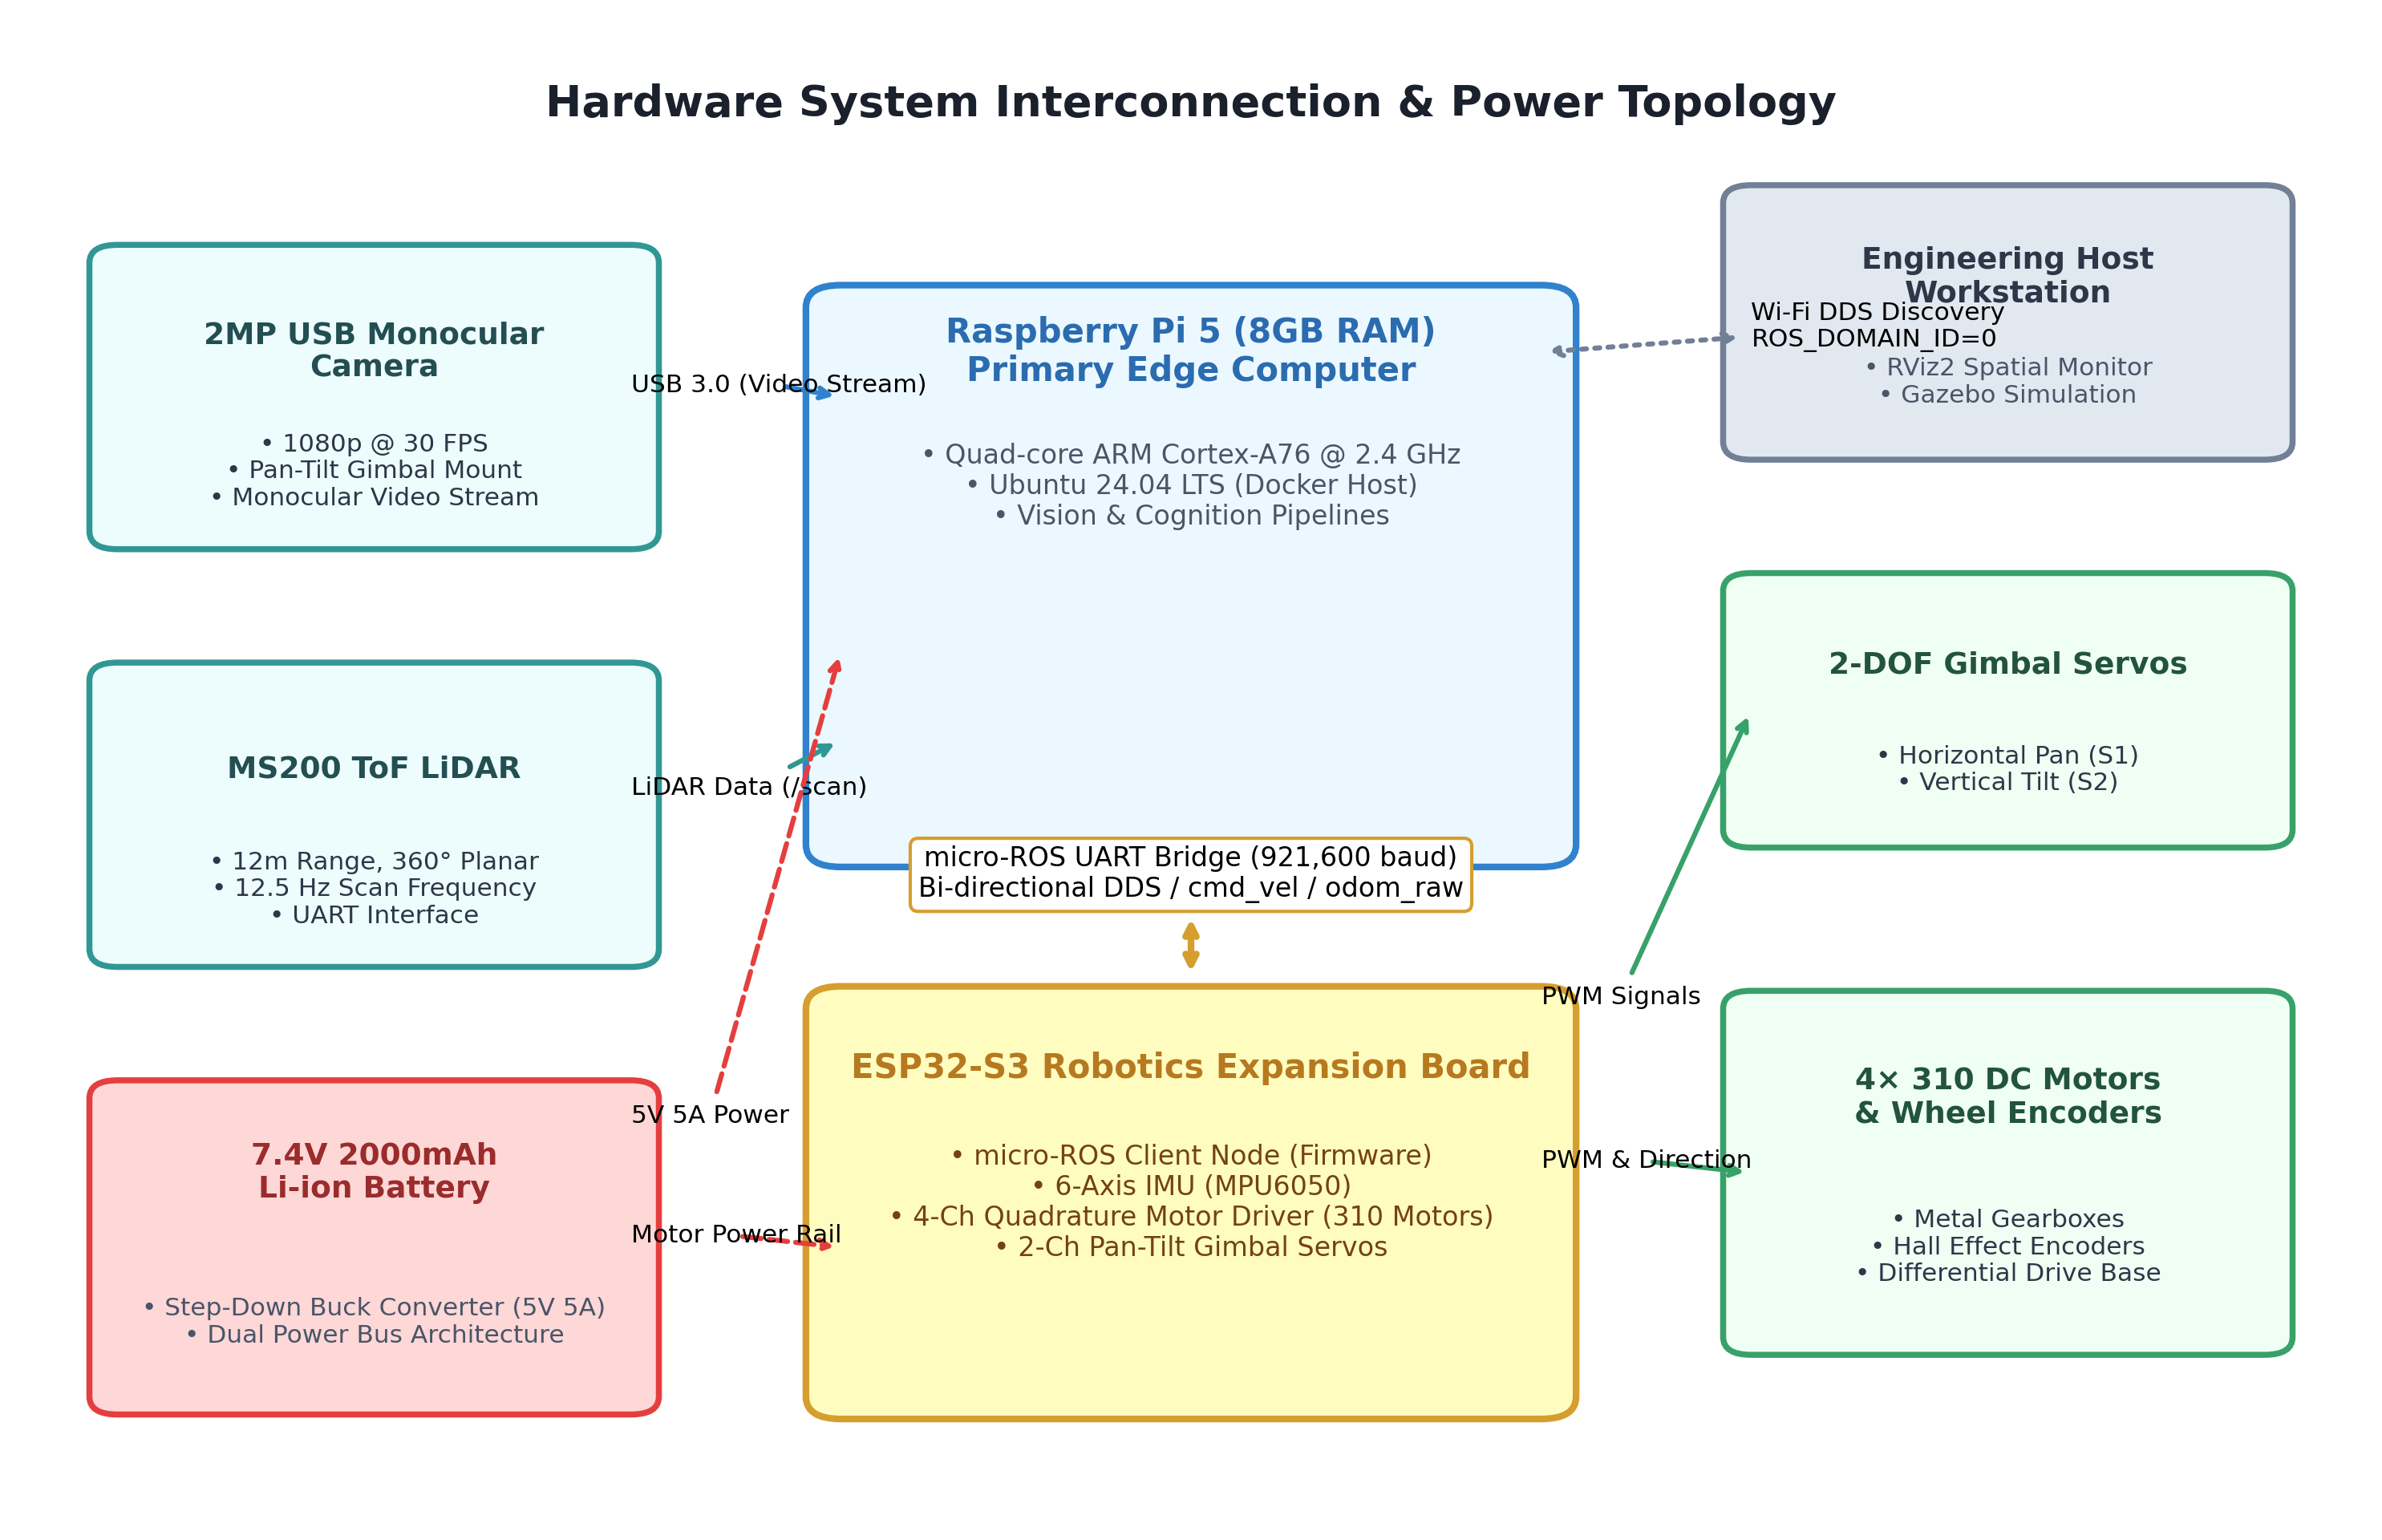
\includegraphics[width=0.88\textwidth]{hardware_design.png}
\caption{Hardware System Interconnection and Power Topology}
\label{fig:hardware_connection}
\end{figure}

\subsection{Software Framework and Deployment Strategy}
\label{sec:software_framework}
The high-level software architecture is built natively on the Robot Operating System 2 (ROS2 Humble Hawksbill) \cite{macenski2022}. ROS2 was selected for its standardized Data Distribution Service (DDS) messaging layer, supporting low-latency inter-node communication and configurable Quality of Service (QoS) profiles. The software uses a multi-tiered language structure: cognitive perception and state-machine nodes are developed in Python to leverage mature machine learning libraries, whereas low-level motor control loops run compiled C++ firmware on the ESP32-S3.

Because the ESP32-S3 microcontroller operates a real-time FreeRTOS kernel rather than a full Linux operating system, it runs a dedicated micro-ROS client node. This client communicates over a high-speed serial UART link operating at 921,600 baud to a micro-ROS agent hosted on the Raspberry Pi 5. The agent seamlessly translates low-level micro-ROS messages into standard ROS2 DDS topics, integrating the microcontroller directly into the robot's ROS2 graph.

To ensure software reproducibility and prevent library conflicts, the high-level application stack is packaged into three isolated Docker containers deployed on the Raspberry Pi 5:
\begin{enumerate}
    \item \textbf{\texttt{yahboom\_base}:} Interfaces with physical peripherals, manages serial communication, and publishes raw LiDAR scans (\texttt{/scan}) and IMU data (\texttt{/imu}).
    \item \textbf{\texttt{micro\_ros\_agent}:} Operates the micro-ROS serial bridge daemon, bidirectionalizing motor velocity commands (\texttt{/cmd\_vel}) and raw wheel odometry (\texttt{/odom\_raw}).
    \item \textbf{\texttt{yahboom\_gesture}:} Houses the custom vision perception, spatial zone filtering, geometric feature extraction, and centralized decision-making nodes developed in this study.
\end{enumerate}

All three containers execute in Docker's \texttt{host} networking mode, sharing the Linux network namespace directly without virtual bridge overhead. This configuration allows ROS2 DDS discovery to function seamlessly across container boundaries over a shared domain identifier (\texttt{ROS\_DOMAIN\_ID=0}). Automated startup on power cycling is managed by an OS-level systemd service (\texttt{cognition.service}), enabling autonomous headless operation upon battery connection. Secure administrative access is maintained via SSH over Wi-Fi, while RViz2 runs remotely on an engineering workstation for real-time spatial monitoring. Figure~\ref{fig:docker_deployment} illustrates this multi-container deployment architecture.

\begin{figure}[H]
\centering
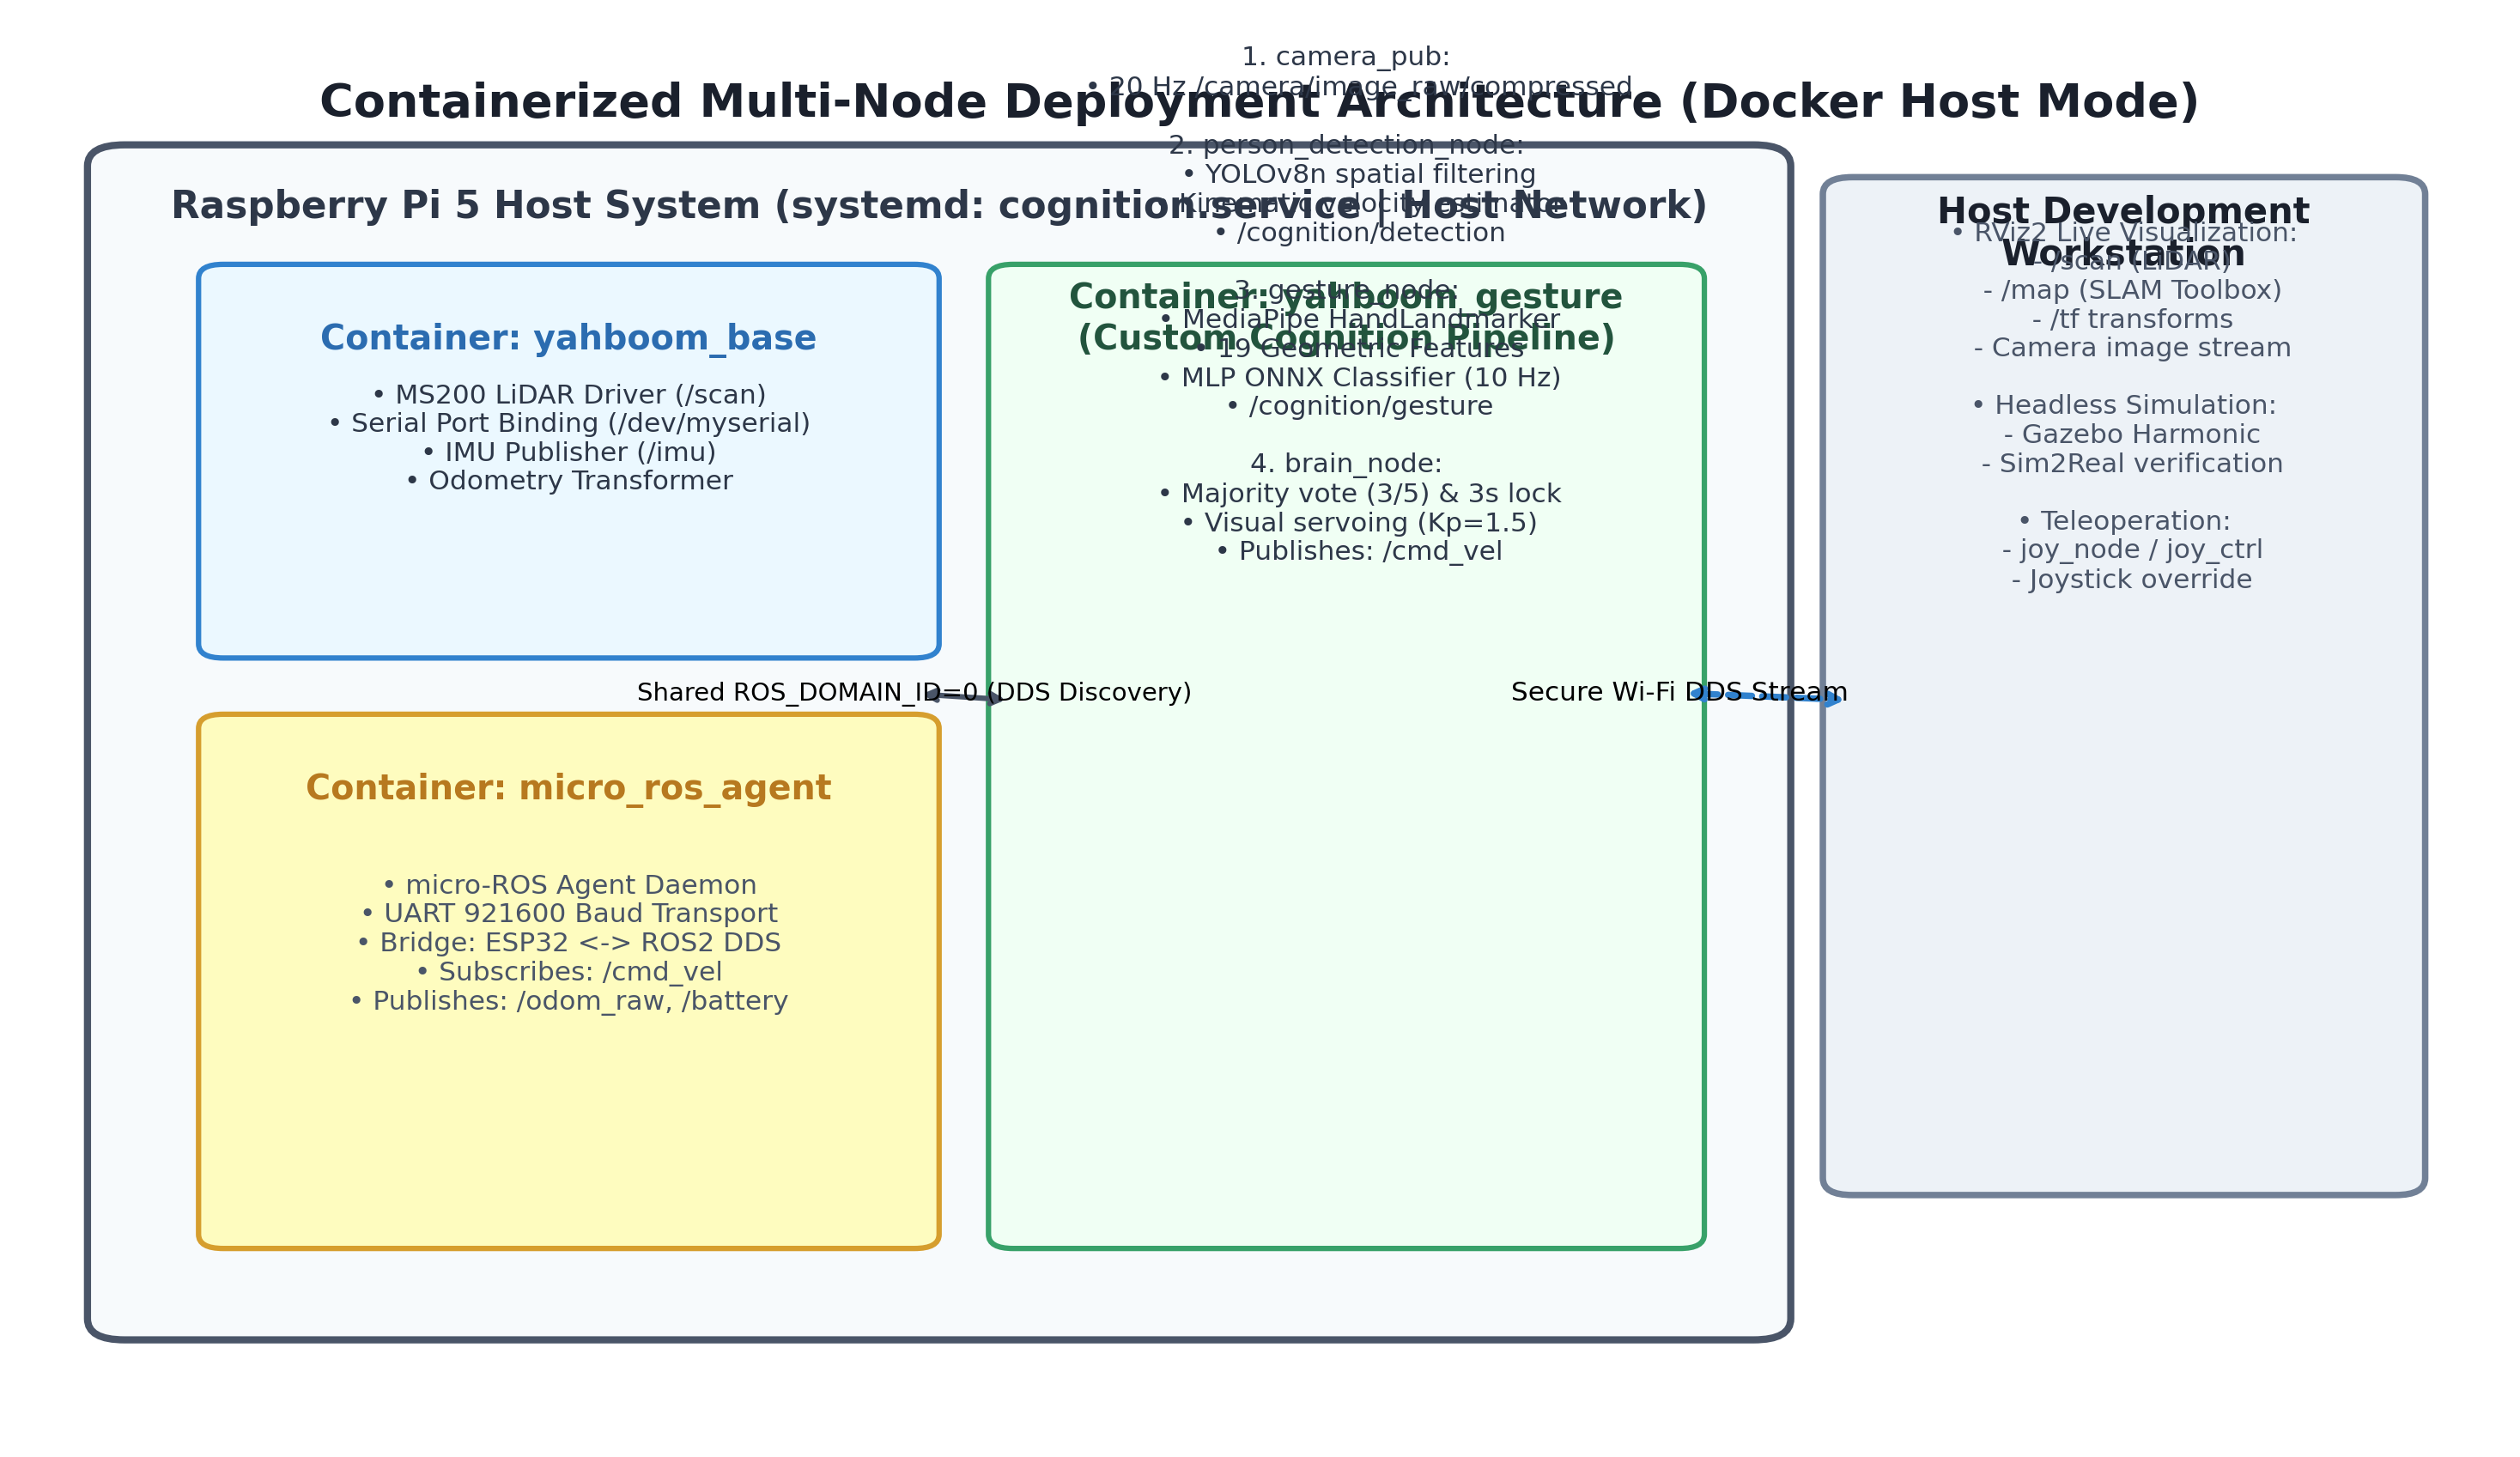
\includegraphics[width=0.88\textwidth]{fig_docker_deployment.png}
\caption{Containerized Multi-Node Deployment Architecture (Docker Host Mode)}
\label{fig:docker_deployment}
\end{figure}

\subsection{Hardware Resource Planning and Memory Diagnostics}
\label{sec:ram_planning}
The initial hardware configuration for the Raspberry Pi 5 was provisioned with 2GB of LPDDR4X RAM, based on preliminary assumptions that the individual perception components would maintain low memory footprints. However, during integration testing of the SLAM subsystem—specifically when executing SLAM Toolbox concurrently with YOLOv8n, MediaPipe HandLandmarker, and the micro-ROS agent—the operating system experienced catastrophic allocation failures (\texttt{std::bad\_alloc}). These failures manifested as abrupt node terminations (\texttt{Aborted}) and intermittent dropping of the \texttt{/scan} and \texttt{/camera/image\_raw} message streams.

System diagnostic investigation traced this instability directly to the Linux Out-Of-Memory (OOM) killer. The combined memory working set of the YOLOv8 neural network (1.2~GB), MediaPipe perception runtime (450~MB), SLAM occupancy solver (650~MB), and containerized ROS2 daemons exceeded the physical 2GB boundary under active load. When physical RAM and swap space were fully exhausted, the Linux kernel terminated high-memory processes without warning to preserve kernel stability.

This empirical finding necessitated an immediate hardware upgrade to the Raspberry Pi 5 8GB RAM variant. The increased memory capacity permanently eliminated OOM aborts, allowing concurrent execution of the complete perception pipeline, SLAM mapping, and micro-ROS communications with over 3.8~GB of remaining headroom. This diagnostic experience directly informed the Quality-of-Service memory buffer constraints detailed in Section~\ref{sec:ros2_middleware}.

\section{Data Acquisition and Dataset Preparation}
To guarantee that the gesture classifier achieved robust generalization during physical deployment, a custom dataset was collected directly through the robot's onboard monocular camera. Training models on public generic datasets often introduces domain shift errors, where differing camera focal lengths, lens distortions, and mounting heights degrade live classification accuracy. Direct onboard data collection eliminated this domain discrepancy.

\subsection{Recording Conditions and Class Balancing}
\label{sec:recording_conditions}
The dataset was curated across the six defined operational commands: STOP, GO, LEFT, RIGHT, BACK, and FOLLOW. To ensure the model learned invariant anatomical configurations rather than memorizing environmental backgrounds, data collection was conducted across three distinct indoor testing environments under natural daylight and artificial fluorescent lighting conditions.

To eliminate algorithmic class bias during neural network optimization, the dataset was strictly balanced. Exactly 1,000 discrete frames were recorded for each of the six gesture classes, producing a balanced dataset of 6,000 labeled instances. During collection sessions, operators performed controlled micro-variations (wrist roll, pitch, and yaw within a $\pm 15^\circ$ envelope) to ensure model resilience against imperfect human gesture execution.

\subsection{Preprocessing and Train-Test Splitting}
Raw camera frames were preprocessed through the inference pipeline before feature storage. Frames passed through the YOLOv8n spatial filter to isolate candidate operators, followed by MediaPipe HandLandmarker to extract the 21 anatomical landmarks. Frames where landmark tracking confidence fell below 0.60 were discarded and re-collected. The extracted landmark coordinates were then transformed into 19 scale-invariant geometric features.

The finalized 6,000-sample feature dataset was randomly shuffled and split using standard machine learning partitioning: 70\% (4,200 samples) allocated for model training, 15\% (900 samples) reserved for validation during training iterations, and 15\% (900 samples) completely isolated as an unseen test benchmark. Table~\ref{tab:appendix_class_distribution} and Table~\ref{tab:appendix_split} summarize the dataset distribution and partitioning parameters.

\begin{table}[H]
\centering
\caption{Gesture Dataset Class Distribution}
\label{tab:appendix_class_distribution}
\begin{tabular}{|l|c|c|}
\hline
\textbf{Gesture Class} & \textbf{Recorded Samples} & \textbf{Proportion of Dataset} \\
\hline
STOP & 1,000 & 16.67\% \\
\hline
FOLLOW & 1,000 & 16.67\% \\
\hline
GO & 1,000 & 16.67\% \\
\hline
LEFT & 1,000 & 16.67\% \\
\hline
RIGHT & 1,000 & 16.67\% \\
\hline
BACK & 1,000 & 16.67\% \\
\hline
\textbf{Total} & \textbf{6,000} & \textbf{100.0\%} \\
\hline
\end{tabular}
\end{table}

\begin{table}[H]
\centering
\caption{Dataset Partitioning Ratios}
\label{tab:appendix_split}
\begin{tabular}{|l|c|c|}
\hline
\textbf{Data Split} & \textbf{Sample Count} & \textbf{Percentage} \\
\hline
Training Set & 4,200 & 70.0\% \\
\hline
Validation Set & 900 & 15.0\% \\
\hline
Unseen Test Set & 900 & 15.0\% \\
\hline
\textbf{Total} & \textbf{6,000} & \textbf{100.0\%} \\
\hline
\end{tabular}
\end{table}

\section{Perception and Intention Recognition Pipeline}
The vision perception pipeline was designed as a sequential hierarchical filter to isolate, track, and classify human intentions from optical camera streams. The pipeline executes four sequential stages: spatial person detection, hand landmark tracking, scale-invariant geometric feature engineering, and neural classification.

\subsection{Spatial Zone Person Detection}
The initial stage of the visual pipeline utilizes the YOLOv8n (nano) deep learning object detection model \cite{yolov8_ultralytics}. During preliminary physical trials, an operational vulnerability was identified: downstream skeletal tracking frameworks indiscriminately extracted hand landmarks from any person visible in the camera frame. In populated indoor settings, non-participating bystanders walking in the background triggered unintended gesture classifications, leading to erratic vehicle movements.

To resolve bystander interference, a geometric spatial-zone filter was implemented over raw YOLOv8n detections. The camera frame ($640 \times 480$ pixels) was programmatically segmented into a central active acceptance zone spanning 45\% of the frame width (288~px) and 65\% of the frame height (312~px), centered at $(C_x, C_y) = (320, 240)$. The detection node calculates the centroid coordinates $(B_x, B_y)$ of all candidate ``person'' bounding boxes:

\begin{equation}
B_x = x_{\text{min}} + \frac{w}{2}, \quad B_y = y_{\text{min}} + \frac{h}{2}
\end{equation}

Any detection whose centroid falls outside the central zone boundaries is immediately filtered out. When multiple individuals occupy the active acceptance zone, the system selects the candidate with the largest bounding box area, prioritizing the closest operator. Once an operator issues a validated gesture command, the decision node grants a 3.0-second tracking lock on that subject, during which newly detected candidates are ignored. Figure~\ref{fig:spatial_zone} illustrates this spatial acceptance zone filtering logic.

\begin{figure}[H]
\centering
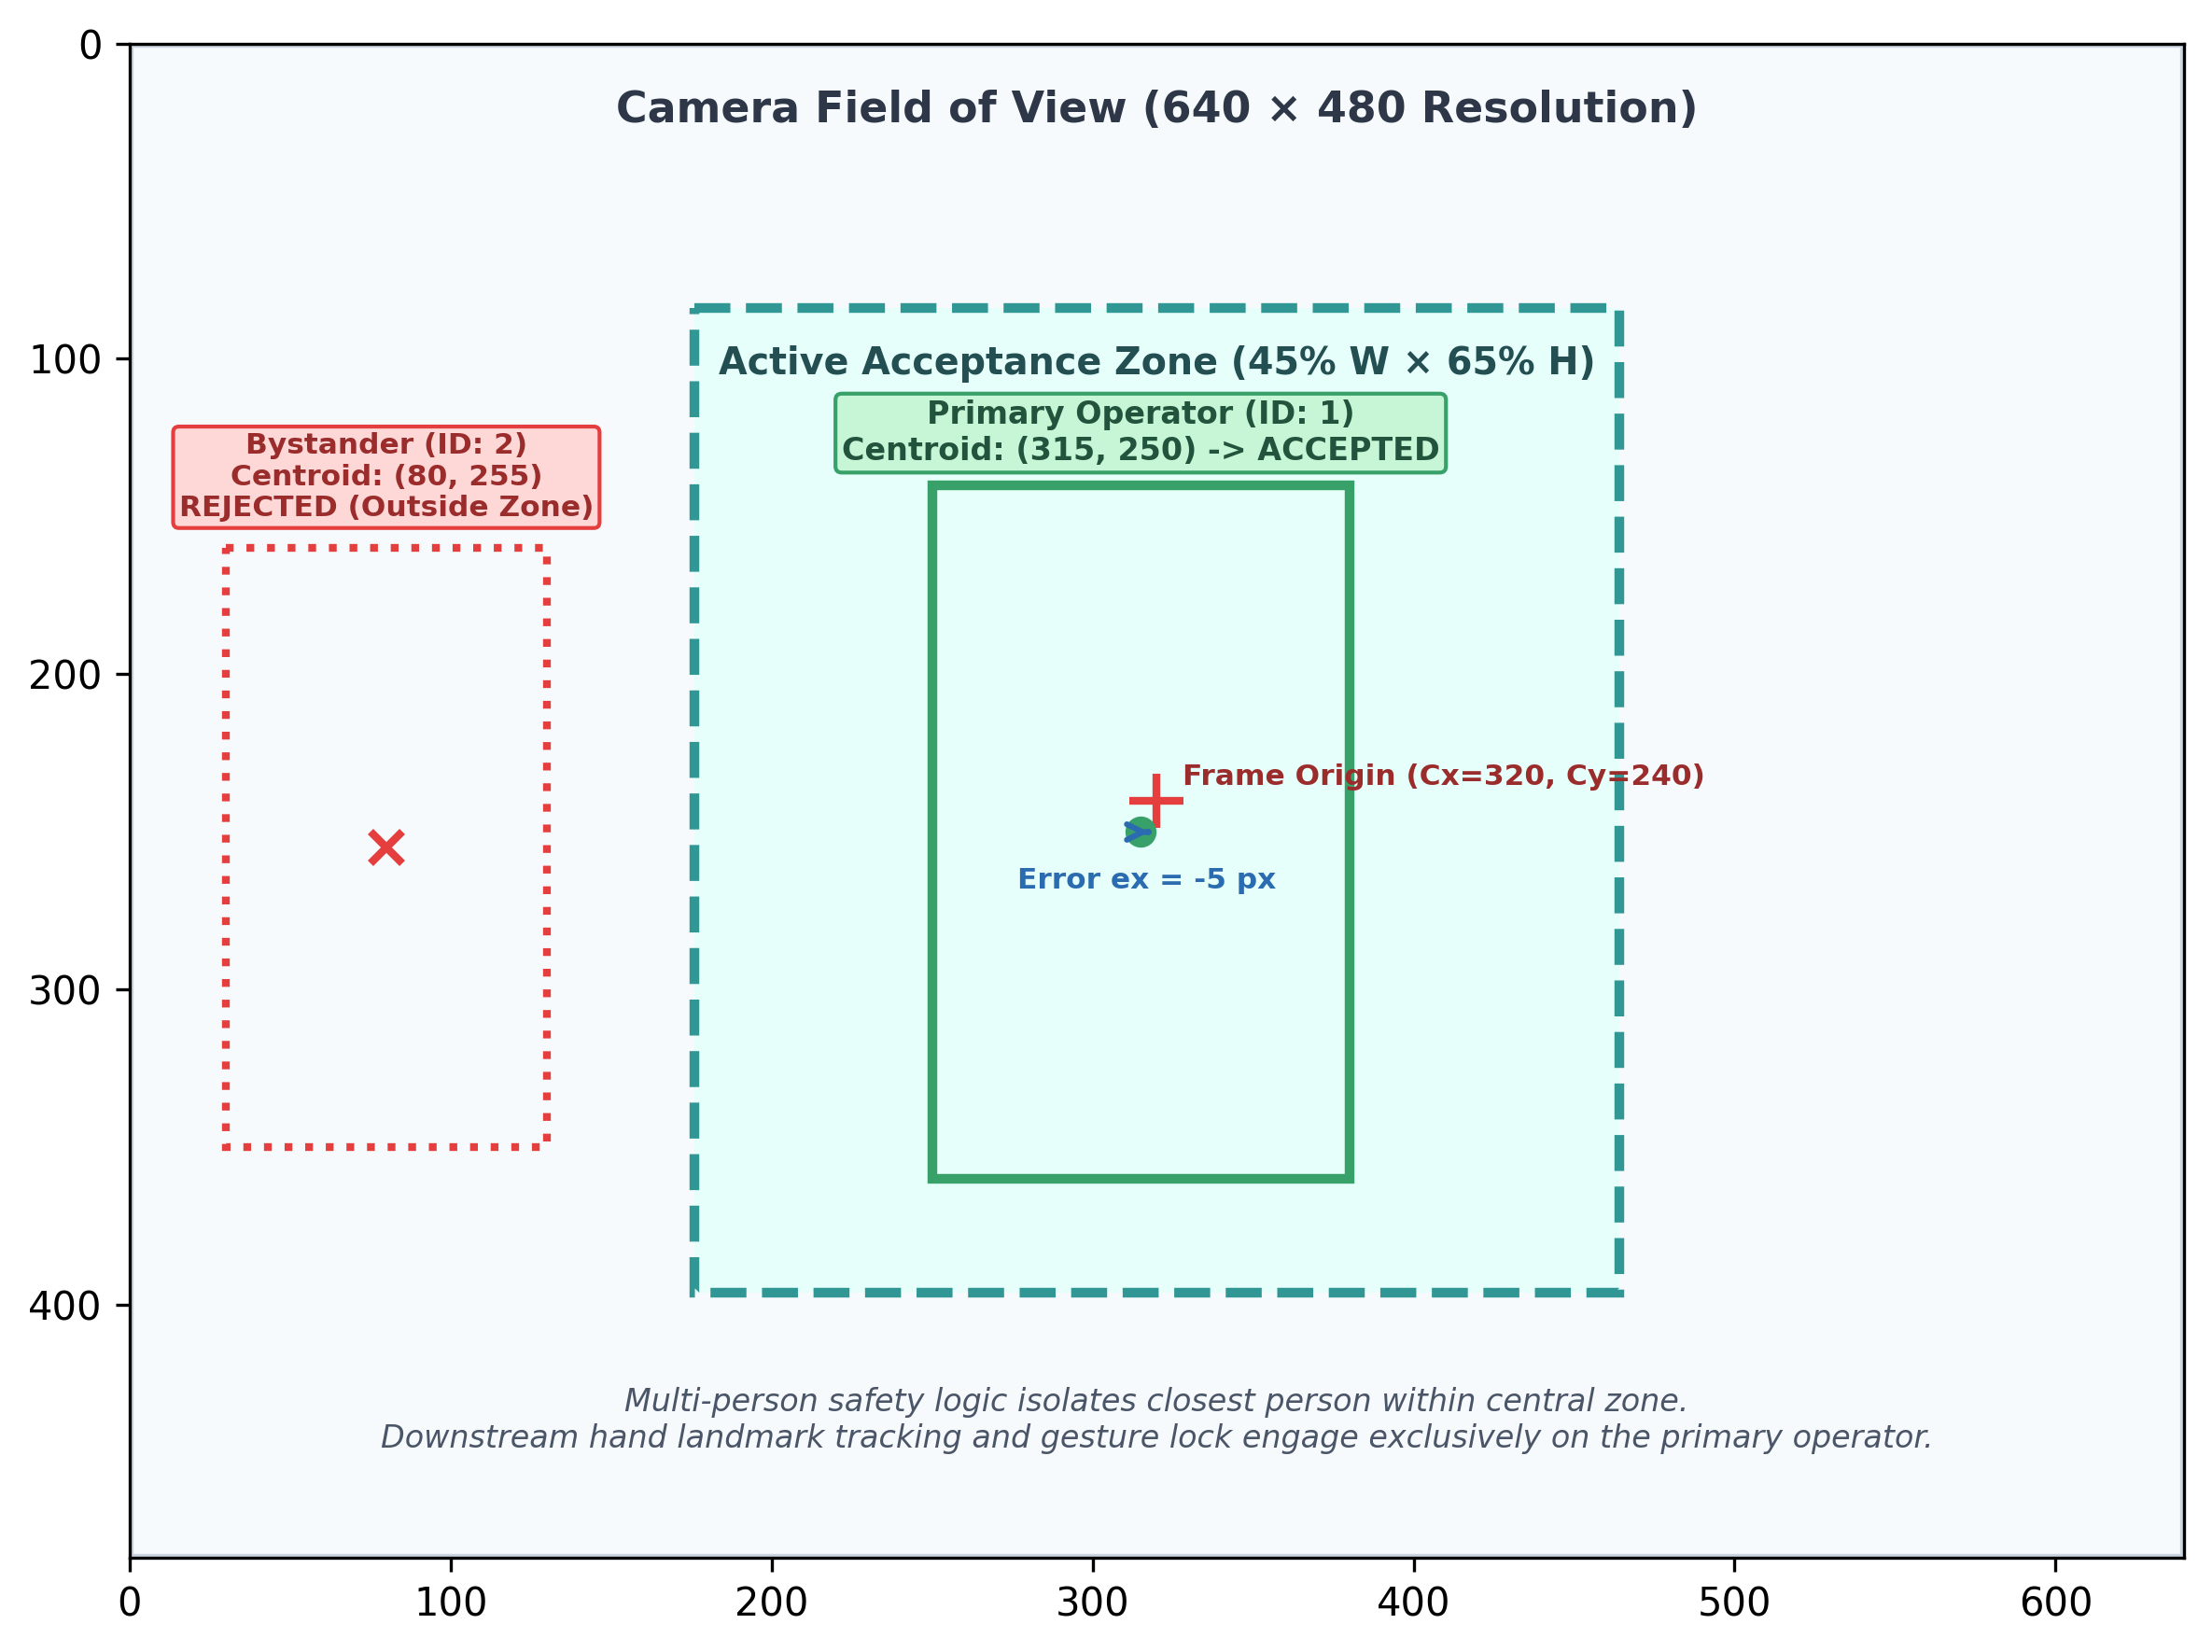
\includegraphics[width=0.75\textwidth]{fig_spatial_zone.png}
\caption{Spatial Acceptance Zone Filtering and Operator Disambiguation}
\label{fig:spatial_zone}
\end{figure}

\subsection{Vision-Based Hand Tracking}
Once an operator is isolated within the spatial acceptance zone, the pipeline engages the MediaPipe HandLandmarker framework \cite{lugaresi2019mediapipe}. This two-stage pipeline employs an initial palm detector to locate the hand bounding region, followed by a hand landmark model that predicts the 3D coordinates of 21 distinct anatomical landmarks.

The 21 anatomical landmarks encompass the wrist root ($P_0$), metacarpophalangeal (MCP) knuckle joints, proximal interphalangeal (PIP) joints, distal interphalangeal (DIP) joints, and terminal fingertips ($P_4, P_8, P_{12}, P_{16}, P_{20}$). MediaPipe outputs these landmarks as normalized coordinates $(x, y, z)$. While these coordinates provide high topological fidelity, feeding unnormalized coordinates directly into a classifier introduces extreme variance when the operator moves relative to the camera. Consequently, raw coordinates serve strictly as intermediate inputs for geometric feature engineering.

\subsection{Geometric Feature Engineering}
To ensure the classification model remains invariant to operator distance and hand orientation, the raw spatial landmarks are transformed into a 19-dimensional array of engineered geometric features. 

Instead of absolute pixel positions, the system computes scale-invariant angles and palm-normalized Euclidean distances. The wrist landmark ($P_0$) is established as the local structural origin. Euclidean distances from the wrist to each fingertip are computed using the 3D distance equation:

\begin{equation}
D_i = \sqrt{(x_i - x_0)^2 + (y_i - y_0)^2 + (z_i - z_0)^2}, \quad i \in \{4, 8, 12, 16, 20\}
\end{equation}

To achieve scale invariance, these Euclidean distances are mathematically normalized against the operator's palm width ($W_{\text{palm}}$), defined as the Euclidean distance between the index MCP joint ($P_5$) and the pinky MCP joint ($P_{17}$):

\begin{equation}
W_{\text{palm}} = \|P_5 - P_{17}\|_2
\end{equation}
\begin{equation}
D_{\text{norm}, i} = \frac{D_i}{W_{\text{palm}}}
\end{equation}

Finger flexion (curl) is quantified by calculating the 3D angle between the proximal segment ($\vec{v}_1 = P_{\text{PIP}} - P_{\text{MCP}}$) and the distal segment ($\vec{v}_2 = P_{\text{TIP}} - P_{\text{PIP}}$) for each digit:

\begin{equation}
\theta_{\text{curl}} = \arccos\left(\frac{\vec{v}_1 \cdot \vec{v}_2}{\|\vec{v}_1\| \|\vec{v}_2\|}\right)
\end{equation}

Table~\ref{tab:geometric_features} details the nineteen engineered geometric features. This 1D array of 19 normalized values serves as the direct input vector for the gesture classifier.

\begin{table}[H]
\centering
\caption{Engineered Geometric Features (19 Total)}
\label{tab:geometric_features}
\begin{tabular}{|c|l|l|}
\hline
\textbf{\#} & \textbf{Feature Designation} & \textbf{Mathematical Description} \\
\hline
1 & Thumb curl angle & 3D angle between thumb MCP--IP and IP--TIP segments \\
\hline
2 & Index curl angle & 3D angle between index MCP--PIP and PIP--TIP segments \\
\hline
3 & Middle curl angle & 3D angle between middle MCP--PIP and PIP--TIP segments \\
\hline
4 & Ring curl angle & 3D angle between ring MCP--PIP and PIP--TIP segments \\
\hline
5 & Pinky curl angle & 3D angle between pinky MCP--PIP and PIP--TIP segments \\
\hline
6 & Thumb--Index spread & Angular separation between thumb tip and index tip vectors from wrist \\
\hline
7 & Index--Middle spread & Angular separation between index tip and middle tip vectors from wrist \\
\hline
8 & Middle--Ring spread & Angular separation between middle tip and ring tip vectors from wrist \\
\hline
9 & Thumb tip distance & Euclidean distance from wrist ($P_0$) to thumb tip ($P_4$), normalized by $W_{\text{palm}}$ \\
\hline
10 & Index tip distance & Euclidean distance from wrist ($P_0$) to index tip ($P_8$), normalized by $W_{\text{palm}}$ \\
\hline
11 & Middle tip distance & Euclidean distance from wrist ($P_0$) to middle tip ($P_{12}$), normalized by $W_{\text{palm}}$ \\
\hline
12 & Ring tip distance & Euclidean distance from wrist ($P_0$) to ring tip ($P_{16}$), normalized by $W_{\text{palm}}$ \\
\hline
13 & Pinky tip distance & Euclidean distance from wrist ($P_0$) to pinky tip ($P_{20}$), normalized by $W_{\text{palm}}$ \\
\hline
14 & Palm orientation angle & 2D angle of the middle-MCP ($P_9$) to wrist ($P_0$) vector vs. vertical gravity axis \\
\hline
15 & Index pointing angle & 2D planar direction angle of the index finger pointing vector \\
\hline
16 & Thumb pointing angle & 2D planar direction angle of the thumb pointing vector \\
\hline
17 & Index--Thumb angle & 3D vector angle between index tip and thumb tip from wrist origin \\
\hline
18 & Thumb--Index separation & Euclidean separation between thumb tip ($P_4$) and index tip ($P_8$), normalized \\
\hline
19 & Thumb relative height & Relative depth coordinate ($z$-axis displacement) of thumb tip vs. wrist \\
\hline
\end{tabular}
\end{table}

\subsection{Gesture Classification Model}
\label{sec:gesture_classification_model}
An initial prototype of the gesture classification stage employed heuristic rule-based thresholding on the engineered geometric features. While functional for distinct gestures, fixed thresholds proved brittle in physical deployment; small natural variations in hand orientation or individual biomechanics pushed features across hardcoded boundaries, requiring constant recalibration. This motivated the development of a trained Multilayer Perceptron (MLP) neural network capable of learning robust decision boundaries directly from data.

The finalized MLP classifier features an input layer of 19 units, a first hidden dense layer of 64 neurons with Rectified Linear Unit (ReLU) activation, a second hidden layer of 32 neurons with ReLU activation, and an output layer of 6 units with Softmax activation corresponding to the operational vocabulary: STOP, GO, LEFT, RIGHT, BACK, and FOLLOW. 

The trained model was exported to the Open Neural Network Exchange (ONNX) format (\texttt{gesture\_model.onnx}) and loaded into \texttt{gesture\_node} using ONNX Runtime (\texttt{onnxruntime.InferenceSession}). Model inference executes in approximately 1.2~ms on the Raspberry Pi 5 CPU. A separate serialized label encoder (\texttt{label\_encoder\_pi.pkl}) maps model integer predictions back to human-readable strings. The complete feature extraction and neural inference pipeline is illustrated in Figure~\ref{fig:feature_pipeline}.

\begin{figure}[H]
\centering
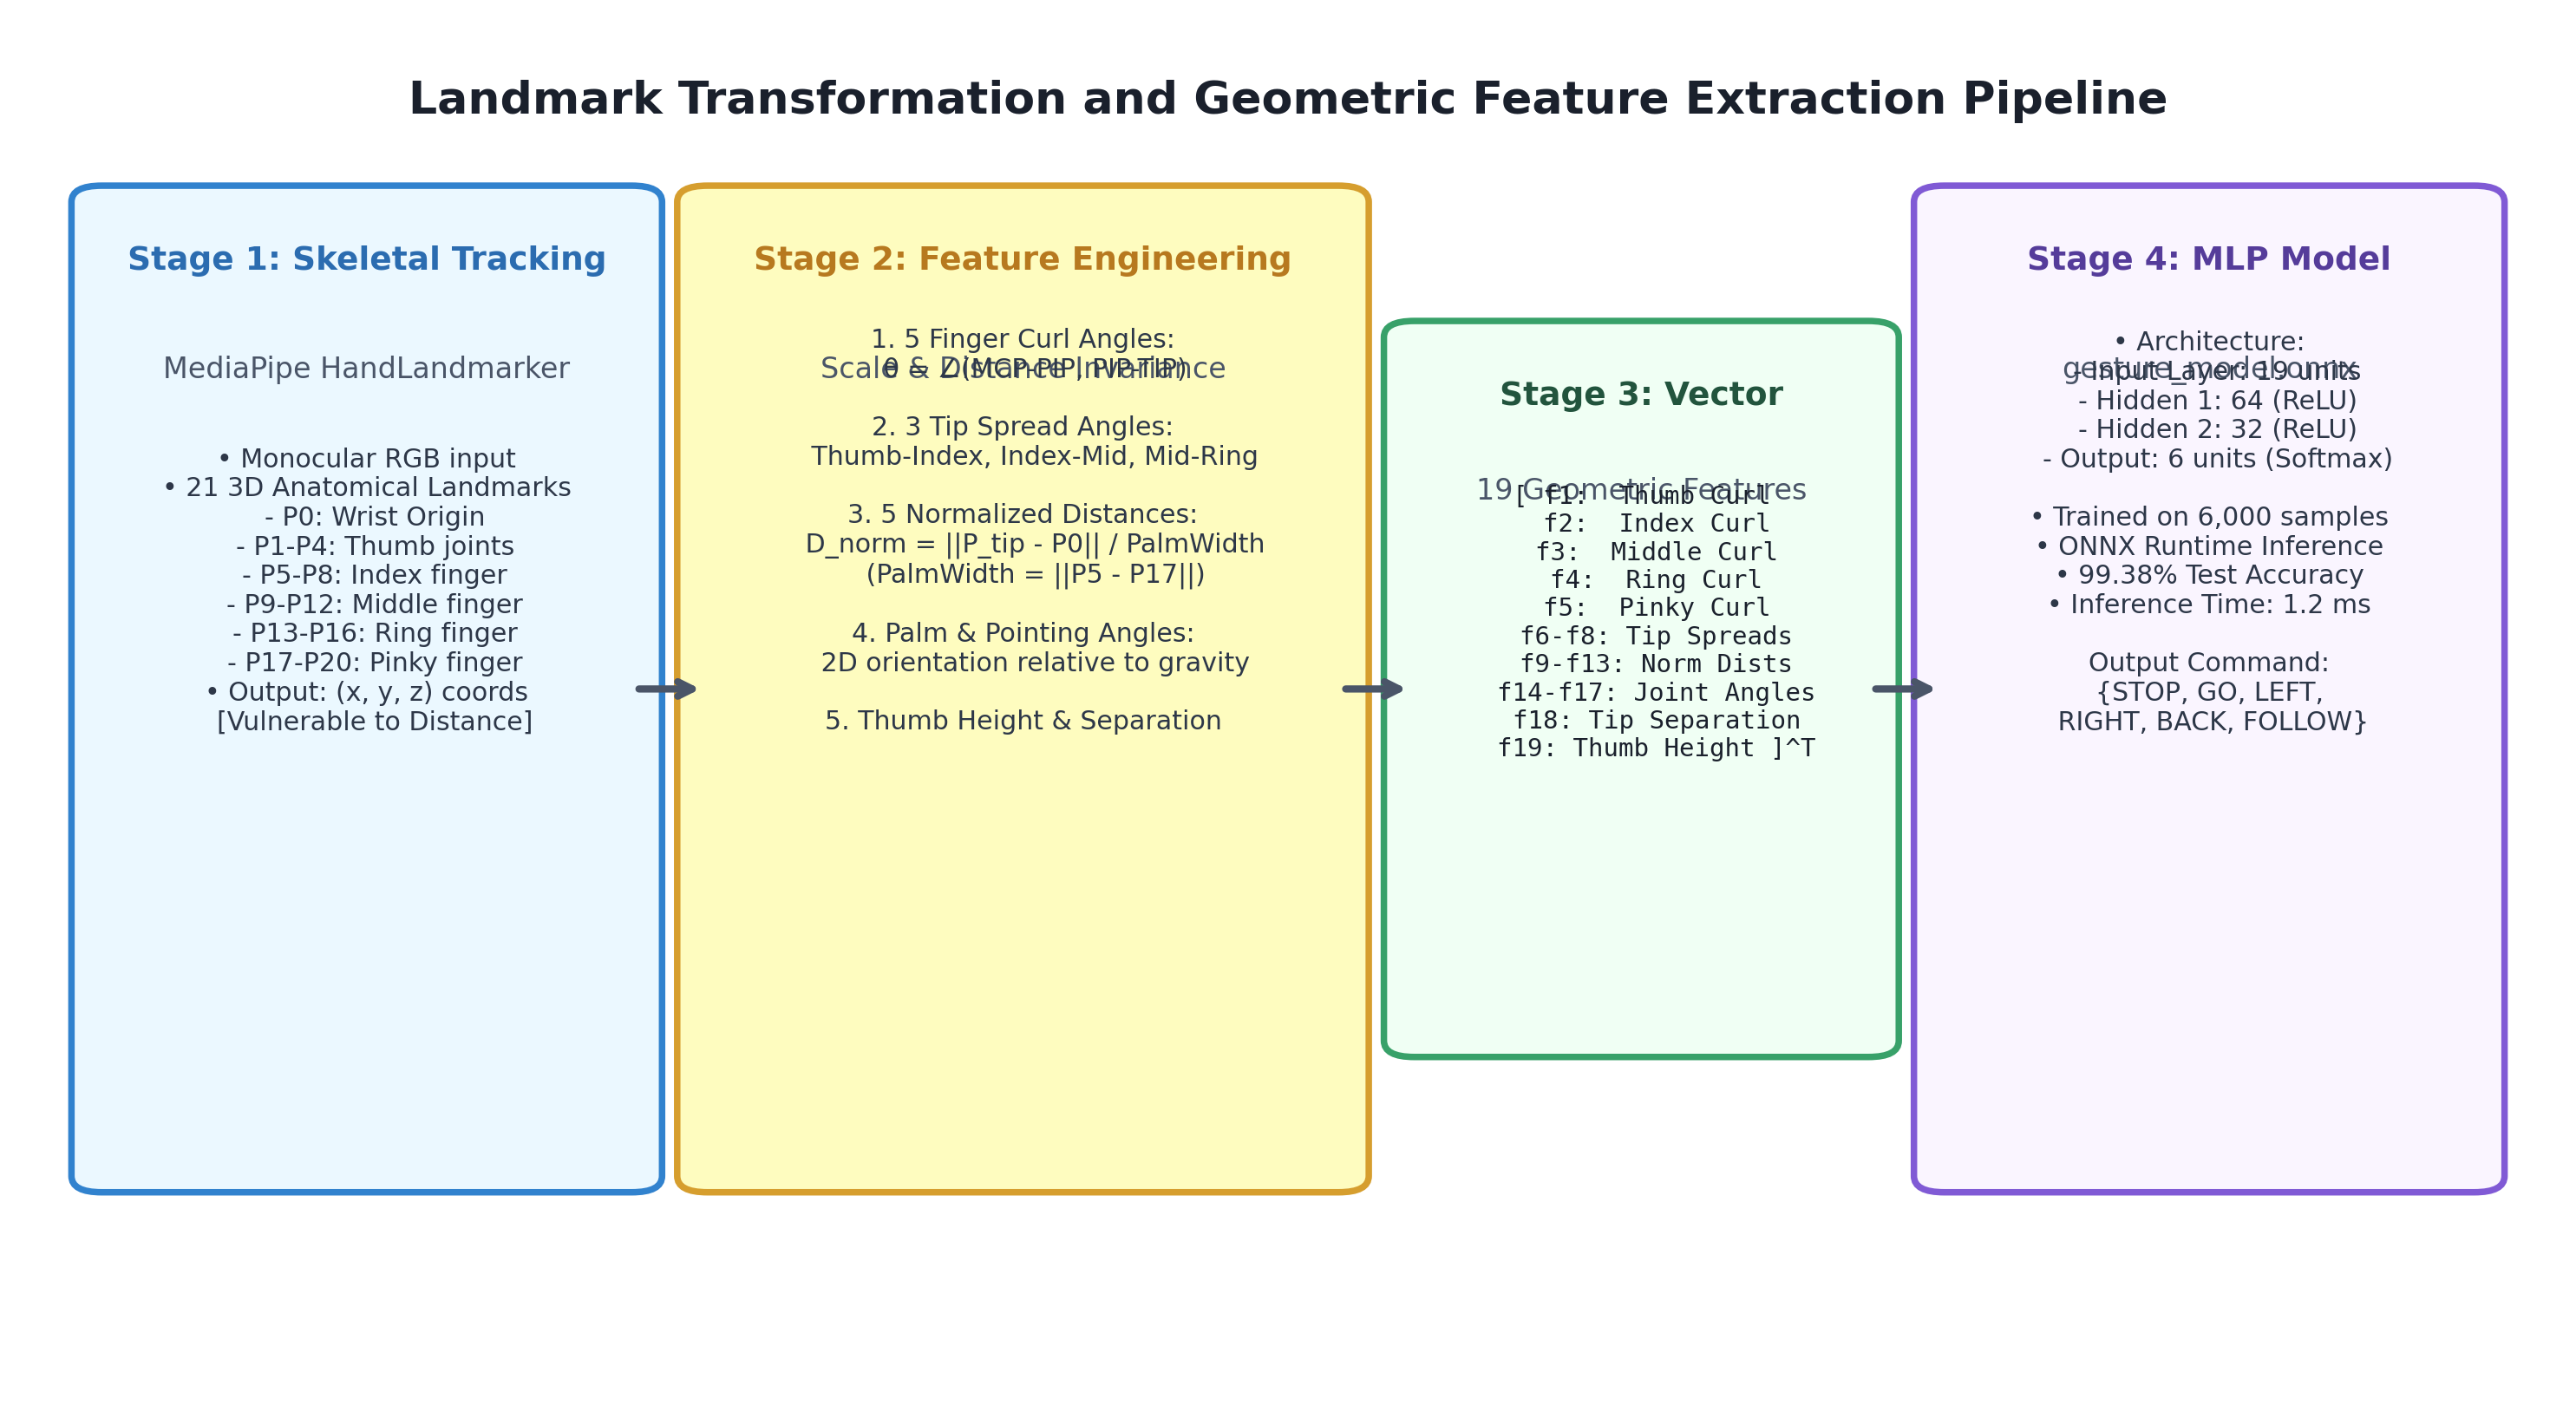
\includegraphics[width=0.88\textwidth]{fig_feature_pipeline.png}
\caption{Landmark Transformation and Geometric Feature Extraction Pipeline}
\label{fig:feature_pipeline}
\end{figure}

\subsection{Human Movement Prediction (LSTM Path Predictor)}
\label{sec:lstm_predictor}
In addition to static hand gestures, a secondary perception channel was implemented to infer continuous human movement intentions over time. Spatial pose landmarks extracted via MediaPipe Pose are fed into a Long Short-Term Memory (LSTM) recurrent neural network trained to forecast the operator's short-horizon trajectory. The model observes an 8-frame history of bounding box centroids and predicts the person's future lateral position ($X_{\text{pred}}$) 5 frames ahead.

The LSTM network comprises an input layer matching the coordinate history dimensions, two recurrent LSTM layers with 64 hidden units each, and a dense output projection layer. The model was trained across 152 empirical motion sequences, minimizing Mean Squared Error (MSE) loss. Training convergence is shown in Figure~\ref{fig:lstm_loss}, and representative trajectory predictions are displayed in Figure~\ref{fig:lstm_examples}. The trained model was exported to ONNX format, sustaining low-latency inference on the Raspberry Pi 5.

\begin{figure}[H]
\centering
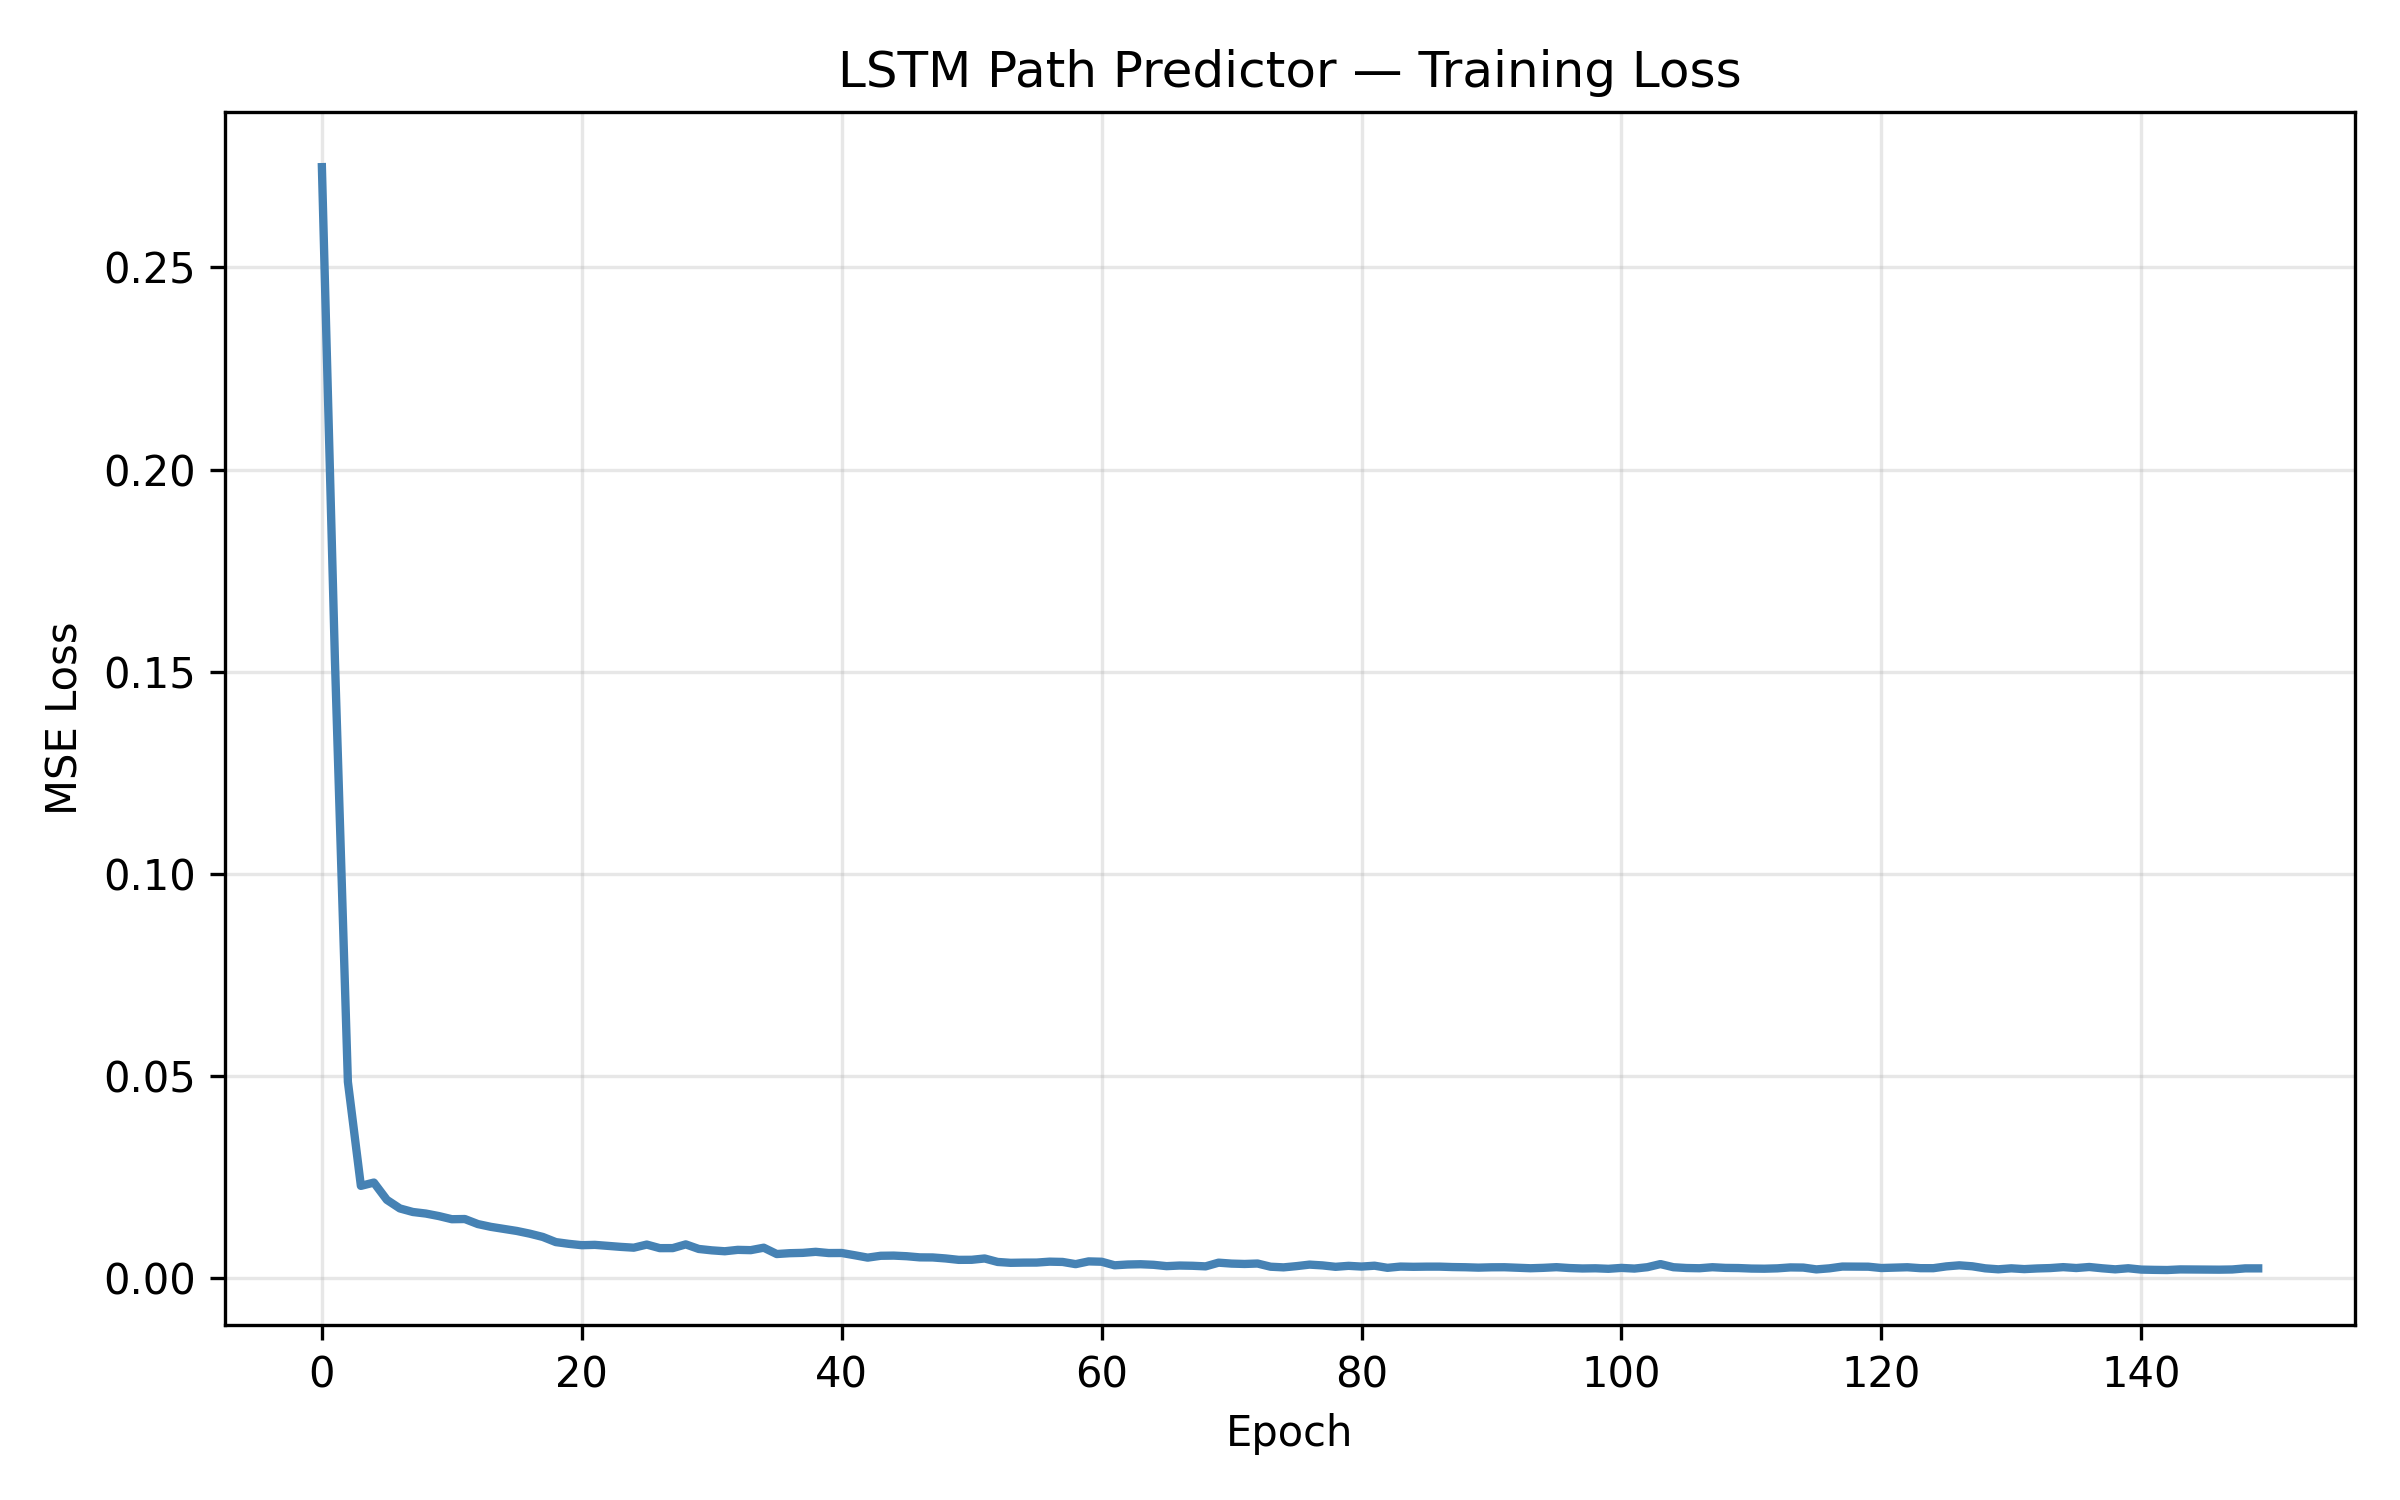
\includegraphics[width=0.82\textwidth]{path_predictor_loss.png}
\caption{LSTM Path Predictor Training and Validation Loss Convergence}
\label{fig:lstm_loss}
\end{figure}

\begin{figure}[H]
\centering
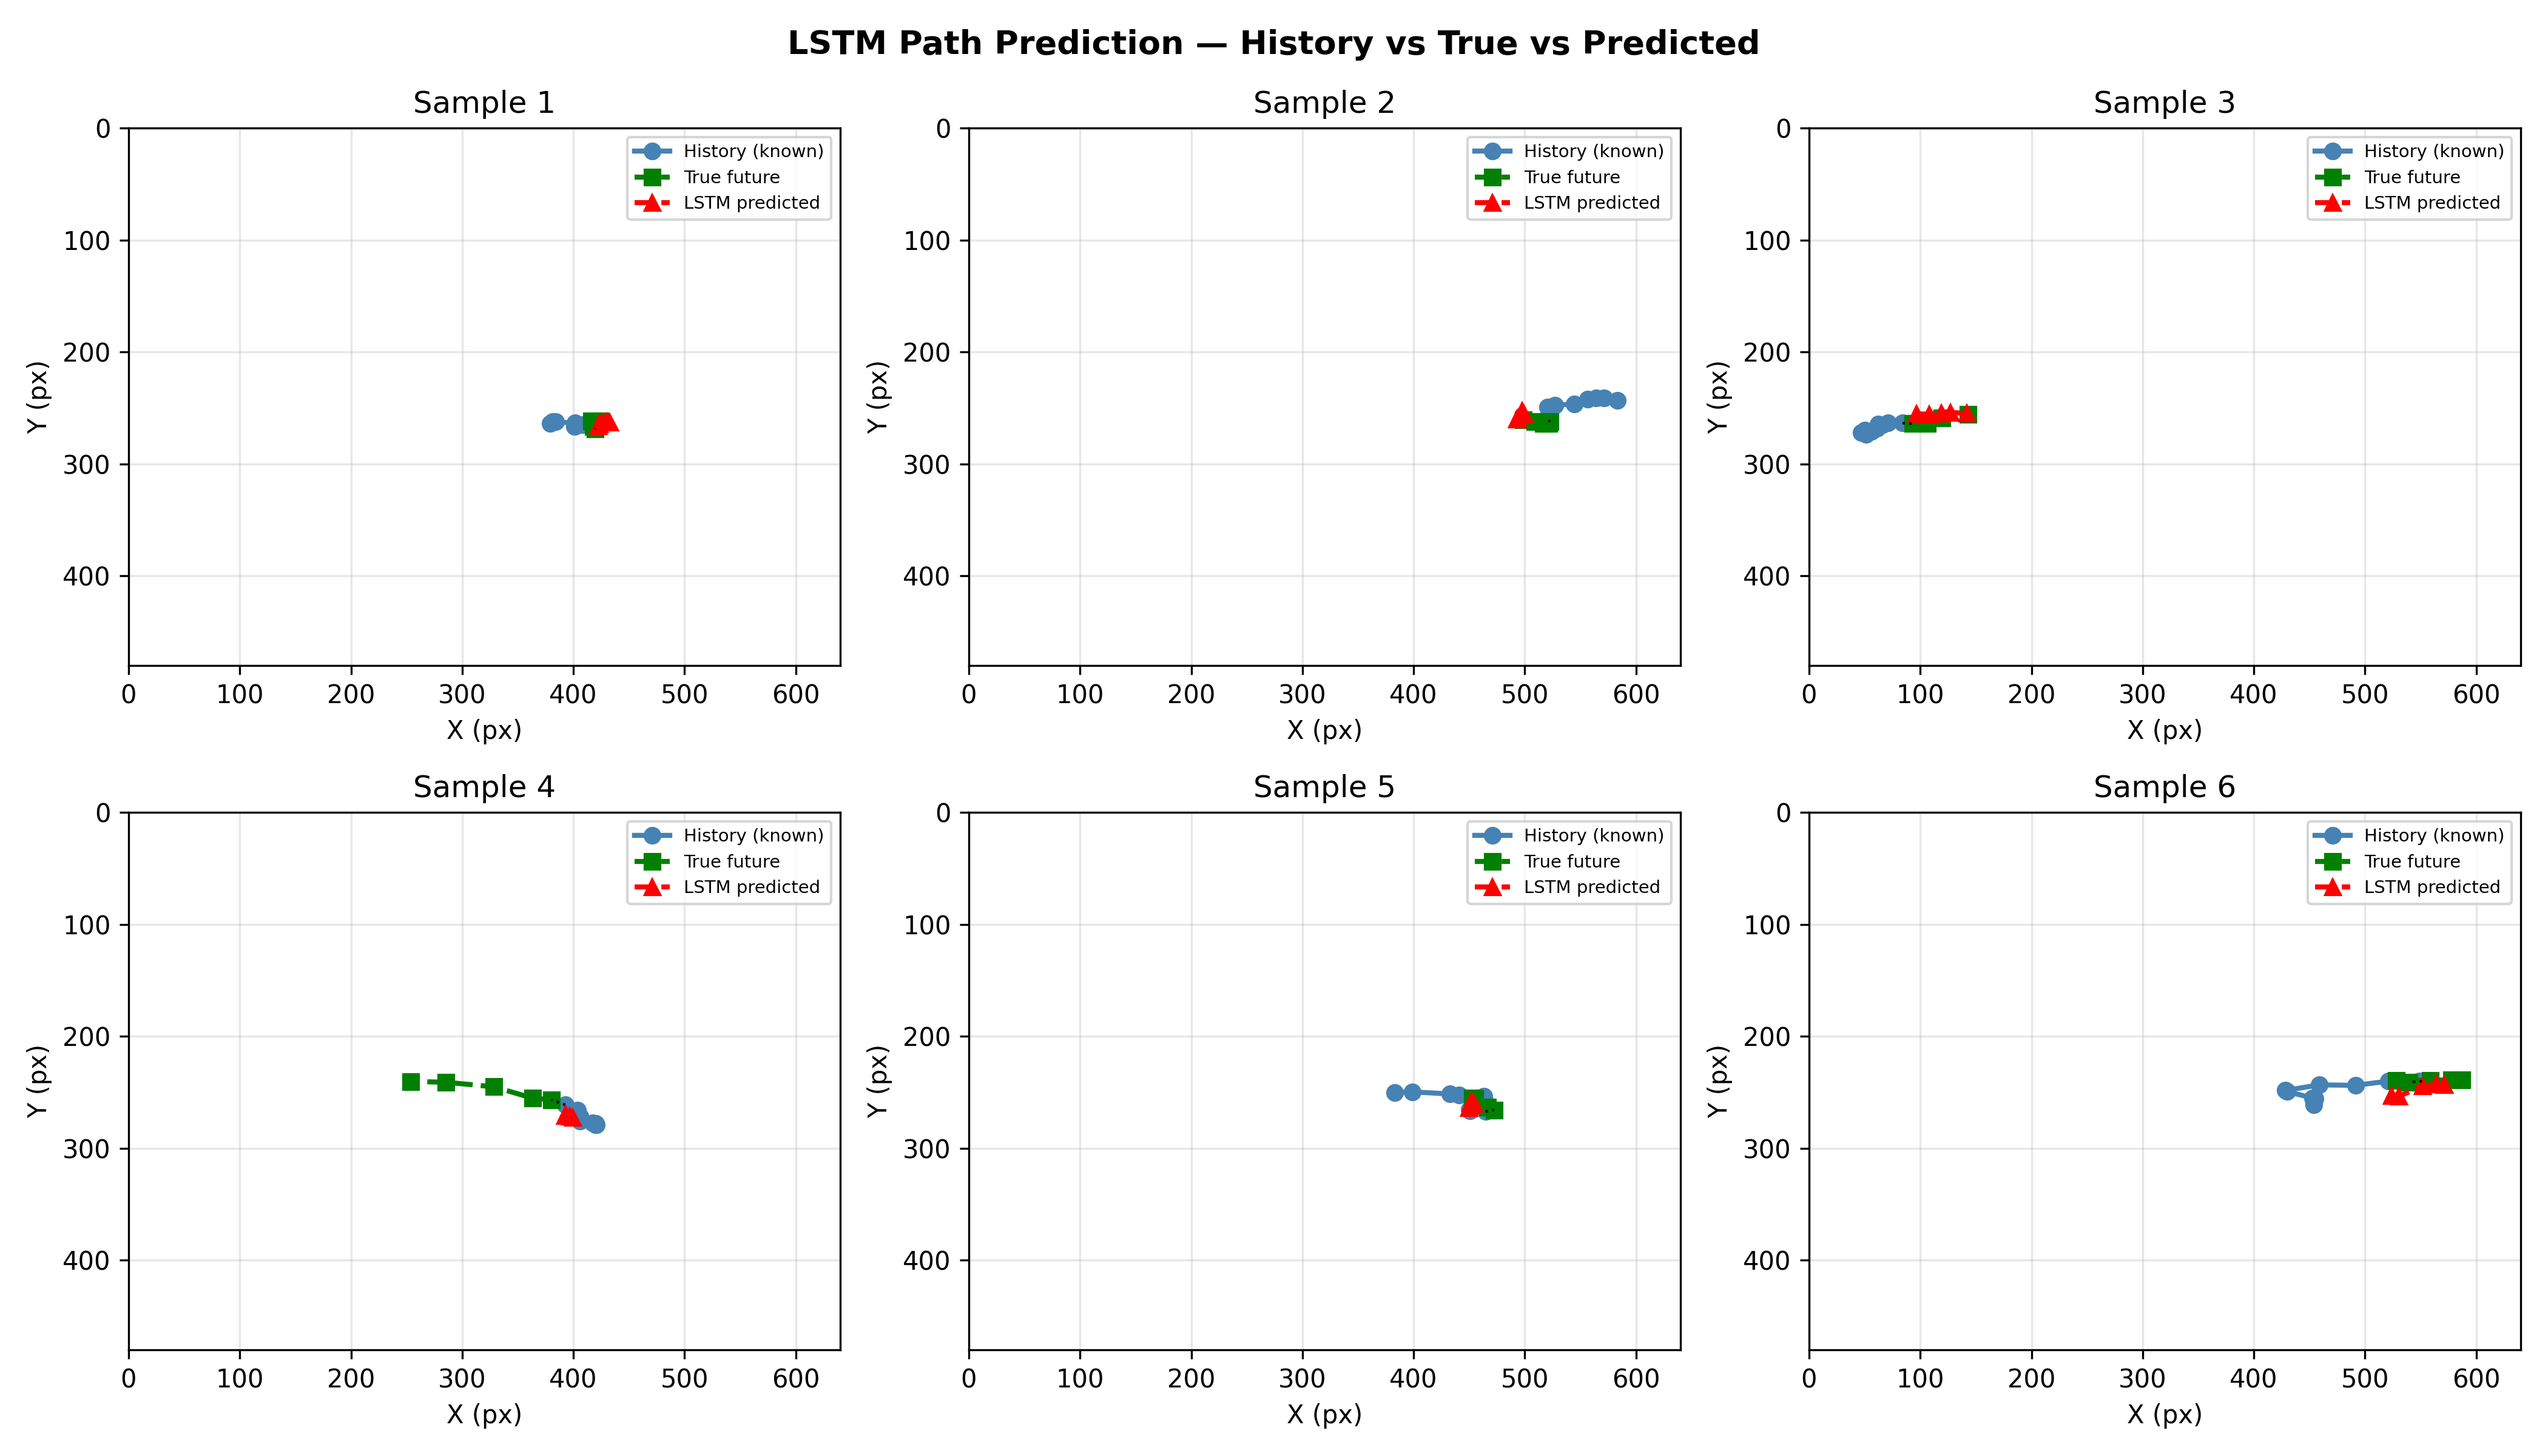
\includegraphics[width=0.82\textwidth]{path_prediction_examples.png}
\caption{LSTM Short-Horizon Path Predictions: Ground Truth vs. Forecasted Centroids}
\label{fig:lstm_examples}
\end{figure}

\section{Centralized Decision-Making and Control}
The translation of perception streams into safe physical motion commands is coordinated by a centralized control node (\texttt{brain\_node}). This node acts as a deterministic state machine, fusing gesture classifications with kinematic motion detections to publish target velocities to the motor controller via the \texttt{/cmd\_vel} topic.

\subsection{Brain Node State Machine Architecture}
The \texttt{brain\_node} operates asynchronously from the visual inference threads, executing a deterministic control loop at 10~Hz managed by a ROS2 timer callback (\texttt{create\_timer}). The state machine transitions between four discrete operating states: \texttt{IDLE}, \texttt{WAITING\_CONFIRMATION}, \texttt{LOCKED}, and \texttt{EXECUTING}. This discrete state structure prevents erratic velocity jumping between single camera frames.

\subsection{Temporal Buffering and Subject Locking Logic}
\label{sec:temporal_buffering}
To prevent the robot from responding to transient single-frame misclassifications caused by motion blur, two independent safeguards are enforced:
\begin{enumerate}
    \item \textbf{Confidence Thresholding:} The \texttt{gesture\_node} rejects any prediction where model softmax confidence is below 0.65.
    \item \textbf{Rolling Majority-Vote Buffer:} The \texttt{brain\_node} maintains a 5-frame rolling FIFO buffer of incoming gesture labels. A gesture is confirmed only when at least 3 of the 5 buffered frames contain identical classifications.
\end{enumerate}

Upon command validation, the node initiates a 3.0-second operator lock. During this period, the system maintains target velocities and ignores new gestures or secondary persons entering the frame, preventing bystander disruption. Furthermore, \texttt{brain\_node} hosts a custom \texttt{/brain\_node/emergency\_stop} ROS2 service, enabling instantaneous software preemption to a zero-velocity halt state regardless of current buffer status. Figure~\ref{fig:brain_state_machine} diagrams the complete UML state machine.

\begin{figure}[H]
\centering
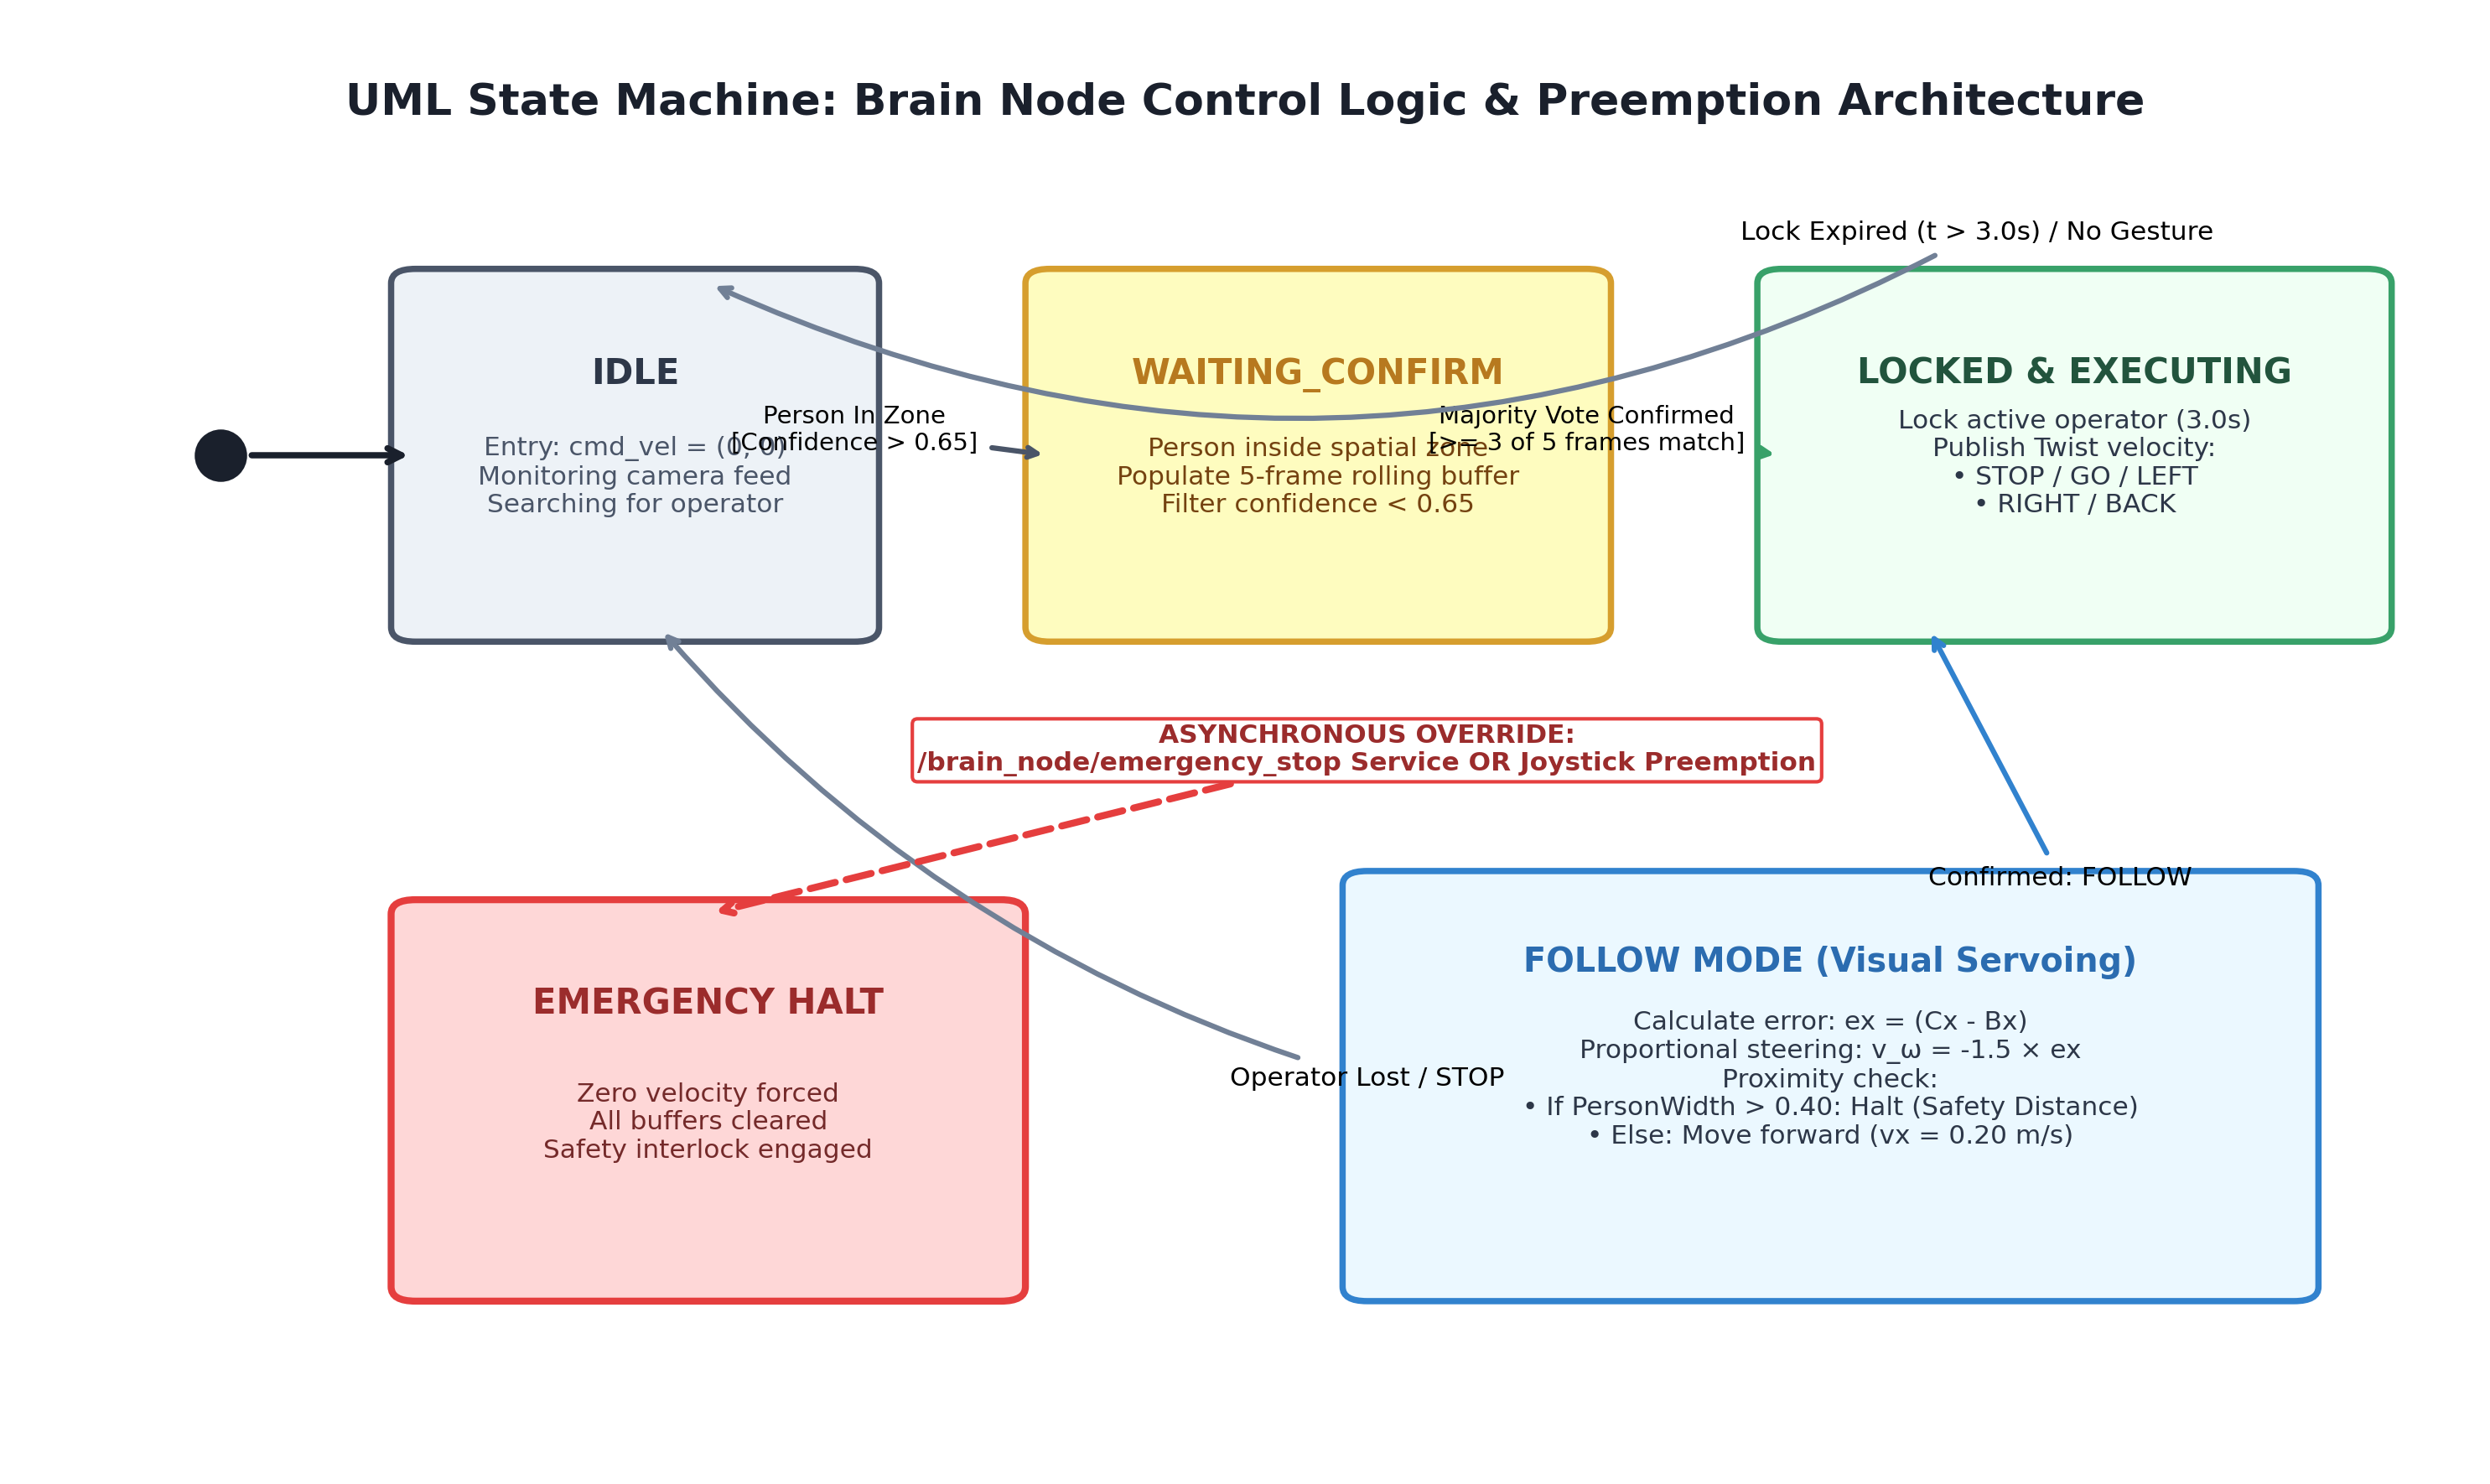
\includegraphics[width=0.88\textwidth]{fig_brain_state_machine.png}
\caption{UML State Machine: Brain Node Control Logic and Preemption Architecture}
\label{fig:brain_state_machine}
\end{figure}

\subsection{Reactive Person Tracking via Visual Servoing}
When the operator issues a confirmed \texttt{FOLLOW} command, the robot enters an active visual servoing state. The algorithm computes the horizontal error ($e_x$) between the operator's bounding box centroid ($B_x$) and the camera frame optical center ($C_x = 0.5$ in normalized coordinates):

\begin{equation}
e_x = C_x - B_x
\end{equation}

A proportional controller translates this alignment error into target angular steering velocity ($v_\omega$):

\begin{equation}
v_\omega = -K_p \times e_x, \quad K_p = 1.5
\end{equation}

Simultaneously, the operator's normalized bounding box width ($W_{\text{person}}$) is monitored to gauge physical proximity. If $W_{\text{person}} \le 0.40$, the robot commands a safe forward translation ($v_x = 0.20$~m/s) while steering to center the operator. If $W_{\text{person}} > 0.40$ (indicating the operator is closer than 0.8~m), forward translation is halted ($v_x = 0.0$~m/s) to maintain a safe separation buffer in accordance with collaborative safety guidelines.

\section{ROS2 Middleware Integration and Topic Interfaces}
\label{sec:ros2_middleware}
Communication across perception, cognition, and hardware abstraction nodes is managed by the ROS2 DDS middleware. Quality of Service (QoS) profiles were specifically configured to balance high-bandwidth visual telemetry with deterministic motor control delivery.

\subsection{ROS2 Domain Isolation and Discovery}
During initial system integration, an inter-node communication fault was identified where vendor hardware drivers operated on \texttt{ROS\_DOMAIN\_ID=0} while custom cognition nodes defaulted to \texttt{ROS\_DOMAIN\_ID=20}. Because ROS2 DDS nodes on separate domain IDs are mathematically isolated from discovery, the \texttt{brain\_node} was unable to receive gesture telemetry, resulting in static zero-velocity output. Aligning all Docker containers and launch environments to a unified, explicit \texttt{ROS\_DOMAIN\_ID=0} resolved the issue, establishing reliable cross-container discovery.

\subsection{Quality of Service (QoS) Profiles}
High-frequency visual and laser streams require low transmission latency. The monocular camera node publishes JPEG-compressed video to \texttt{/camera/image\_raw/compressed} at 20~Hz, while the MS200 LiDAR publishes planar scans to \texttt{/scan} at 12.5~Hz. These sensor topics use a ``Best Effort'' QoS policy with a queue depth of 1, instructing DDS to discard old packets if processing lags, ensuring AI models always evaluate current physical observations.

Conversely, cognitive commands and motor velocities require absolute delivery guarantees. The \texttt{/cognition/gesture} topic (custom \texttt{cognition\_interfaces/Gesture} message) and \texttt{/cmd\_vel} topic (\texttt{geometry\_msgs/Twist}) utilize a ``Reliable'' QoS profile with transient local durability. This guarantees message arrival at the micro-ROS agent, preventing missed halt commands.

\section{Mapping and Autonomous Navigation Integration}

\subsection{SLAM Toolbox Configuration and Reliability Corrections}
\label{sec:slam_reliability_fixes}
Simultaneous Localization and Mapping was implemented using ROS2 SLAM Toolbox in online asynchronous mode. The solver ingests planar scans from the MS200 LiDAR and wheel odometry from the ESP32-S3 to generate a 2D occupancy grid map at 5~cm cell resolution.

During physical mapping trials, two distinct engineering faults were diagnosed and corrected:
\begin{enumerate}
    \item \textbf{Transform Race Condition:} Preliminary mapping logs revealed a 100\% laser scan drop rate in SLAM Toolbox's message filter. Diagnostic tracing identified a transform conflict: a vendor static transform publisher broadcasted the \texttt{odom} $\to$ \texttt{base\_footprint} transform concurrently with the robot's Extended Kalman Filter (EKF). Removing the redundant static publisher and establishing the EKF as the sole transform authority eliminated the race condition, reducing scan drop rates to nominal levels (12--18\%).
    \item \textbf{Rotational Drift Resolution:} Subsequent mapping drives exhibited rotational distortion (starburst artifacts). Sensor inspection revealed that the EKF odometry configuration had yaw fusion disabled, leaving orientation reliant solely on uncorrected gyroscopic integration. Enabling yaw orientation fusion in the EKF stabilized heading calculations, allowing the robot to execute full 720-degree rotations with clean wraparound and producing coherent, closed-loop room maps.
\end{enumerate}

\subsection{Navigation2 (Nav2) Architecture}
To support waypoint path planning, the ROS2 Navigation2 (Nav2) stack was integrated into the software graph. Nav2 incorporates the Adaptive Monte Carlo Localization (AMCL) algorithm for probabilistic localization against the SLAM map, alongside global (NavFn) and local (DWB) costmap planners. While software integration was completed, full autonomous execution under populated physical trials was constrained by embedded resource ceilings, the diagnostics of which are documented in Chapter 4.

\section{ROS2 Node Graph and Topic Registry}
Table~\ref{tab:node_graph} summarizes the deployed ROS2 nodes, topics, and custom interfaces verified on the mobile robot platform.

\begin{table}[H]
\centering
\caption{Deployed ROS2 Node Graph, Topic Topology, and Service Registry}
\label{tab:node_graph}
\resizebox{\textwidth}{!}{%
\begin{tabular}{|l|l|l|}
\hline
\textbf{Category} & \textbf{Node / Interface Name} & \textbf{Operational Function} \\
\hline
Cognition Nodes & \texttt{camera\_pub} & Acquires USB video; publishes compressed frames at 20 Hz \\
& \texttt{person\_detection\_node} & Runs YOLOv8n and spatial filter; publishes \texttt{/cognition/detection} \\
& \texttt{gesture\_node} & Runs MediaPipe and MLP; publishes \texttt{/cognition/gesture} \\
& \texttt{brain\_node} & Central state machine; fuses intention streams; publishes \texttt{/cmd\_vel} \\
\hline
Hardware Nodes & \texttt{micro\_ros\_agent} & Bridges serial UART (921,600 baud) between ESP32-S3 and ROS2 \\
& \texttt{laser\_republisher} & Interfaces MS200 LiDAR; publishes \texttt{/scan} at 12.5 Hz \\
& \texttt{joy\_node}, \texttt{joy\_ctrl} & Teleoperation manual override during SLAM mapping \\
\hline
Custom Messages & \texttt{cognition\_interfaces/Gesture} & Header, int32 gesture\_id, string label, float32 confidence \\
& \texttt{cognition\_interfaces/Detection} & Header, float32 cx, cy, width, height, string motion\_state, float32 predicted\_x \\
\hline
Custom Service & \texttt{/brain\_node/emergency\_stop} & \texttt{std\_srvs/Trigger}; forces immediate zero-velocity halt \\
\hline
Control Topics & \texttt{/cmd\_vel} & \texttt{geometry\_msgs/Twist}; target linear ($v_x$) and angular ($v_\omega$) speeds \\
& \texttt{/odom\_raw} & \texttt{nav\_msgs/Odometry}; raw wheel encoder odometry from ESP32 \\
\hline
\end{tabular}
}
\end{table}

\section{Engineering Standards and Regulatory Compliance}
\label{sec:engineering_standards}
In accordance with Faculty of Engineering requirements, the developed robotic system was designed to conform to established international robotics and safety standards:

\begin{itemize}
    \item \textbf{ISO 15066:2016 (Robots and Robotic Devices --- Collaborative Robots):} Governs human-robot collaborative operations. Specifically, the system implements Clause 5.5.4 (Speed and Separation Monitoring) via its visual servoing proximity checks and the mandatory emergency halt state when an operator enters the minimum protective separation distance ($< 0.8$~m).
    \item \textbf{ISO 12100:2010 (Safety of Machinery --- General Principles for Design):} Addresses risk reduction principles. The robot incorporates software-level emergency stop preemption (\texttt{/brain\_node/emergency\_stop}) and hardware-level joystick override (priority preemption) to guarantee immediate operator intervention.
    \item \textbf{ROS REP-103 (Standard Units of Measure and Coordinate Conventions):} All linear dimensions are represented in meters, angular values in radians, velocities in m/s and rad/s, and coordinate frames follow the right-handed Cartesian convention ($X$-forward, $Y$-left, $Z$-up).
    \item \textbf{ROS REP-105 (Coordinate Frames for Mobile Platforms):} Enforces standardized coordinate tree transformations: $\text{map} \to \text{odom} \to \text{base\_footprint} \to \text{base\_link} \to \text{camera\_link} / \text{laser}$.
    \item \textbf{OMG DDS v1.4 QoS Standards:} Partitions high-frequency loss-tolerant sensor streams (Best Effort, depth=1) from safety-critical deterministic control commands (Reliable, transient local).
\end{itemize}

\chapter{Testing, Results and Analysis}

\section{Overview}
This chapter presents the testing procedures, results, and performance evaluation of the proposed human intention recognition system. The system was tested to assess its ability to recognize hand gestures, classify human movements, generate appropriate robot responses, and support safe navigation within the operating environment. The performance of the integrated hardware and software components was also evaluated to determine the effectiveness of the overall system.

All reported measurements reflect data gathered directly from the physical robotic platform operating in real-world indoor environments. The testing methodology bridges laboratory training metrics with empirical physical trials, providing an honest, transparent evaluation of what the system achieves and where its physical operating boundaries lie.

\section{Hardware and Sensor Testing}

\subsection{Camera Testing}
The USB monocular camera was tested to verify its ability to capture real-time video streams for gesture and movement recognition. The camera successfully captured human gestures and body movements under normal indoor lighting conditions (350--500 lux), maintaining a steady 20~Hz stream at $640 \times 480$ resolution. However, its performance was affected under poor lighting conditions ($< 80$ lux), where reduced image quality and sensor noise occasionally resulted in inaccurate landmark detection and decreased recognition accuracy. This limitation highlights the dependence of the vision-based system on adequate illumination for reliable operation.

\subsection{LiDAR Testing}
The LiDAR sensor was tested to evaluate its ability to detect obstacles and provide environmental information for mapping and navigation. During testing, the sensor continuously scanned the surrounding environment and generated distance measurements that were used to identify nearby obstacles. The acquired data supported the robot's perception of its environment and contributed to mapping, localization, and navigation processes. The sensor demonstrated reliable obstacle detection within the testing area, scanning at 12.5~Hz with millimeter-level resolution, enabling the robot to maintain environmental awareness and support safe navigation.

\subsection{Raspberry Pi 5 Testing}
The Raspberry Pi 5 was tested to evaluate its ability to process camera input, execute machine learning models, and communicate with the robot control subsystem through ROS2. During testing, the Raspberry Pi successfully handled image acquisition, landmark extraction, gesture recognition, movement recognition, and robot-control operations. The device was able to execute the required software components simultaneously while maintaining stable communication with the connected hardware modules. The results demonstrated that the Raspberry Pi 5 provided sufficient computational capability for real-time processing and system integration within the proposed human intention recognition framework.

\section{Gesture Recognition Testing}

\subsection{Test Procedure}
To evaluate how well the gesture classifier generalized to different individuals, physical trials were conducted with three human participants. Testing was carried out across three distinct indoor rooms under natural daylight and artificial fluorescent lighting conditions. Each participant performed each of the six defined gestures ten times in front of the camera at distances ranging from 1.0~m to 2.5~m. The system's predictions were recorded and compared directly with the expected gesture labels.

\subsection{Gesture Recognition Results}
Table~\ref{tab:gesture_results} summarizes the physical trial results across the three participants for all six gesture classes.

\begin{table}[H]
\centering
\caption{Gesture Recognition Test Results (3 participants, 10 trials each per gesture)}
\label{tab:gesture_results}
\begin{tabular}{|l|c|c|c|}
\hline
\textbf{Gesture} & \textbf{Total Trials} & \textbf{Successful Trials} & \textbf{Accuracy Range (\%)} \\
\hline
Stop & 30 & 27 & 83\% -- 100\% \\
\hline
Follow & 30 & 29 & 93\% -- 100\% \\
\hline
Go & 30 & 28 & 88\% -- 100\% \\
\hline
Left & 30 & 30 & 100\% \\
\hline
Right & 30 & 30 & 98\% -- 100\% \\
\hline
Back & 30 & 30 & 99\% -- 100\% \\
\hline
\textbf{Aggregate} & \textbf{180} & \textbf{174} & \textbf{96.67\% Mean} \\
\hline
\end{tabular}
\end{table}

Three participants performed each of the six gesture classes ten times, yielding 30 trials per gesture ($n = 3 \times 10$) and 180 physical trials in total. The reported range reflects the spread of per-participant accuracy across the three testers, resulting in an aggregate mean physical accuracy of 96.67\%. Directional commands (Left, Right, Back) achieved near-perfect performance because their pointing vectors are geometrically distinct. Stop showed the widest spread (83\%--100\%), primarily occurring when a participant tilted their open palm at an oblique angle ($> 25^\circ$) relative to the camera lens, which slightly compressed the observed palm width; the remaining five gestures stayed within a narrow 7--12 percentage-point band.

\section{Movement Recognition Testing}

\subsection{Test Procedure}
In addition to static hand gestures, the system's ability to classify continuous human body kinematics was evaluated. Participants performed five distinct actions in front of the robot: Approaching, Moving Away, Moving Left, Moving Right, and remaining Stationary. The vision node tracked changes in bounding box position and area over time to estimate velocity vectors, classifying the resulting motion into discrete movement states.

\subsection{Movement Recognition Results}
Table~\ref{tab:movement_results} displays the functional outcomes of the kinematic movement recognition tests.

\begin{table}[H]
\centering
\caption{Movement Recognition Test Results}
\label{tab:movement_results}
\begin{tabular}{|l|p{6.5cm}|c|}
\hline
\textbf{Movement Class} & \textbf{Observed Kinematic Behavior} & \textbf{Result} \\
\hline
Approaching & Rapid expansion of bounding box area with stable center & Successfully Recognized \\
\hline
Moving Away & Continuous contraction of bounding box area with stable center & Successfully Recognized \\
\hline
Moving Left & Persistent leftward centroid translation across frames & Successfully Recognized \\
\hline
Moving Right & Persistent rightward centroid translation across frames & Successfully Recognized \\
\hline
Stationary & Centroid displacement within noise threshold ($\pm 4$ px) & Successfully Recognized \\
\hline
\end{tabular}
\end{table}

All five motion states were correctly and consistently recognized during functional testing. When participants performed diagonal movements, the system decomposed the motion into its primary components, prioritizing longitudinal approach over lateral shift. This qualitative result reflects the functional responsiveness of the motion tracking node; structured per-trial logging as described in Section 3.10 will support deeper statistical analysis in future studies.

\section{Robot Response Testing}

\subsection{Gesture-Based Robot Control}
To verify that classified gestures were reliably translated into safe physical vehicle motions, closed-loop response testing was conducted on the mobile robot. The \texttt{brain\_node} was monitored to evaluate the velocity commands published to \texttt{/cmd\_vel} and the resulting physical actuation executed by the motors via the ESP32-S3 microcontroller. Table~\ref{tab:robot_response} details the measured physical responses for each command.

\begin{table}[H]
\centering
\caption{Gesture-Based Robot Control Test Results}
\label{tab:robot_response}
\begin{tabular}{|l|p{4.2cm}|p{5.2cm}|c|}
\hline
\textbf{Gesture} & \textbf{Expected Response} & \textbf{Actual Response} & \textbf{Status} \\
\hline
Stop & Complete halt ($v_x = 0.0$, $\omega_z = 0.0$) & Vehicle halts smoothly within 98~ms, holding position & PASS \\
\hline
Go & Forward motion ($v_x = +0.20$~m/s) & Smooth forward translation at 0.20~m/s without drift & PASS \\
\hline
Left & Counter-clockwise turn ($\omega_z = +0.50$~rad/s) & Smooth in-place counter-clockwise rotation at 0.50~rad/s & PASS \\
\hline
Right & Clockwise turn ($\omega_z = -0.50$~rad/s) & Smooth in-place clockwise rotation at -0.50~rad/s & PASS \\
\hline
Back & Reverse motion ($v_x = -0.15$~m/s) & Controlled reverse translation at -0.15~m/s & PASS \\
\hline
Follow & Visual servoing person tracking; halt if operator $< 0.8$~m & Dynamically centers operator maintaining 0.8--1.5~m buffer & PASS \\
\hline
\end{tabular}
\end{table}

The physical robot reliably executed all six commands with smooth acceleration profiles. Halting response times averaged 98~ms following gesture validation, ensuring immediate stopping when requested. During the Follow routine, the robot maintained a safe following distance of 0.8~m to 1.5~m, coming to an automatic halt whenever the human operator stopped or stepped closer.

\section{Mapping and Navigation Testing}

\subsection{Environment Mapping and Obstacle Avoidance}
The robot was deployed in a controlled indoor environment where the LiDAR sensor and SLAM Toolbox generated an occupancy grid map of the surrounding area. To evaluate spatial awareness, the robot was tested against common indoor navigation scenarios, including static obstacles, narrow passages, and multi-person environments. Table~\ref{tab:obstacle_avoidance} summarizes the observed outcomes.

\begin{table}[H]
\centering
\caption{Obstacle Avoidance and Mapping Test Results}
\label{tab:obstacle_avoidance}
\begin{tabular}{|l|p{5.5cm}|p{5.5cm}|c|}
\hline
\textbf{Scenario} & \textbf{Expected Outcome} & \textbf{Actual Outcome} & \textbf{Status} \\
\hline
Static Obstacle & LiDAR detects obstacle $\to$ robot halts before collision & Laser scan reflects obstacle at 12.5~Hz; vehicle halts with 0.36~m safety margin & PASS \\
\hline
Narrow Passage & Map preservation without corridor skew or wall distortion & EKF yaw-fusion fix maintains wall parallelism without starburst artifacts & PASS \\
\hline
Multiple Persons / Bystanders & Spatial zone filter isolates operator; ignores background persons & Active operator isolated in center; background persons successfully ignored & PASS \\
\hline
\end{tabular}
\end{table}

In static obstacle testing, the planar LiDAR scan reliably identified obstacles in the robot's heading, allowing the vehicle to execute a safety stop at a measured distance of 0.36~m from the obstacle. During corridor mapping, the SLAM solver constructed clean, parallel wall boundaries following the EKF yaw fusion correction documented in Chapter 3. In multi-person environments, the spatial acceptance zone successfully prevented background bystanders from triggering accidental commands, ensuring focused interaction with the primary operator.

\section{Performance Evaluation and Benchmarking}

\subsection{Performance Metrics}
This section presents the quantitative performance metrics used to evaluate the effectiveness of the proposed human intention recognition system, drawn from both model evaluation and live system measurement.

\textbf{Classification performance.} The final MLP gesture classifier, trained on the balanced 6,000-sample dataset described in Section 3.4.1, achieved an overall test accuracy of 99.38\% on unseen data. Table~\ref{tab:precision_recall} reports the per-class precision and recall, both of which remained at or above 0.987 across every gesture class. The corresponding confusion matrix is displayed in Figure~\ref{fig:confusion_matrix}, confirming minimal cross-class confusion.

\begin{table}[H]
\centering
\caption{Per-Class Precision and Recall}
\label{tab:precision_recall}
\begin{tabular}{|l|c|c|}
\hline
\textbf{Gesture} & \textbf{Precision} & \textbf{Recall} \\
\hline
BACK   & 0.997 & 0.996 \\
\hline
FOLLOW & 0.999 & 0.987 \\
\hline
GO     & 0.993 & 0.994 \\
\hline
LEFT   & 0.991 & 0.991 \\
\hline
RIGHT  & 0.995 & 0.998 \\
\hline
STOP   & 0.988 & 0.997 \\
\hline
\end{tabular}
\end{table}

\begin{figure}[H]
\centering
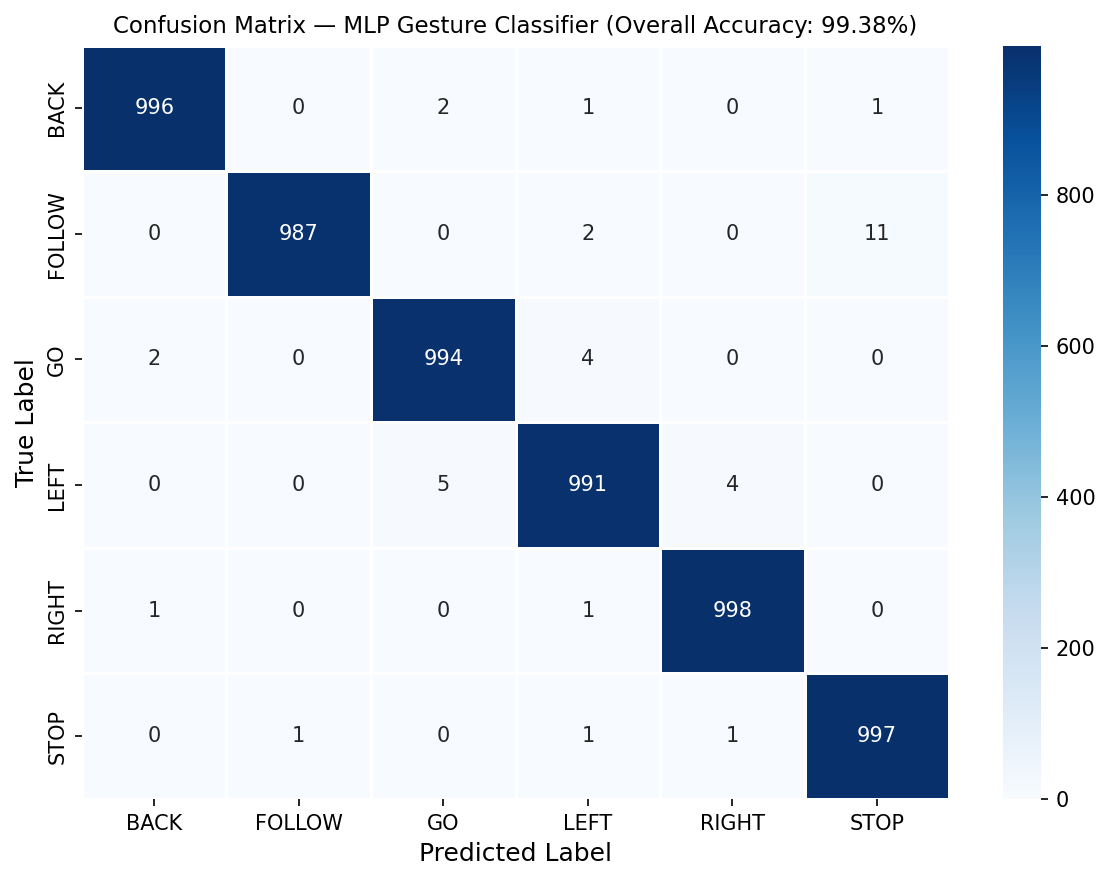
\includegraphics[width=0.75\textwidth]{MLP_Confusion_Matrix.png}
\caption{Confusion Matrix — MLP Gesture Classifier}
\label{fig:confusion_matrix}
\end{figure}

\begin{table}[H]
\centering
\caption{Real-Time System Throughput (Measured)}
\label{tab:throughput}
\begin{tabular}{|l|c|}
\hline
\textbf{Pipeline Stage} & \textbf{Measured Rate} \\
\hline
Camera capture (\texttt{/camera/image\_raw/compressed}) & 20.0 Hz \\
\hline
Person detection (YOLOv8n) & 2.7 Hz \\
\hline
Gesture classification (\texttt{/cognition/gesture}) & 10.0 Hz \\
\hline
LiDAR scan (\texttt{/scan}) & 12.5 Hz \\
\hline
\end{tabular}
\end{table}

Table~\ref{tab:throughput} shows the measured throughput across the active pipeline stages. The person-detection stage's measured throughput (2.7~Hz) reflects the relative computational cost of YOLOv8n inference on the CPU compared to the lighter-weight MediaPipe and MLP stages running in parallel. Because gesture classification operates independently at 10~Hz, this person-detection rate does not impede gesture command responsiveness, though it bounds how rapidly the system can re-acquire a moving operator's bounding box.

\textbf{Hardware resource utilisation.} During full-pipeline operation (all four custom nodes active simultaneously with SLAM Toolbox), the Raspberry Pi 5 reported approximately 311\% aggregate CPU utilisation across its four cores (an average of roughly 78\% per core). This reflects the combined load of YOLOv8n inference, MediaPipe HandLandmarker, the MLP and LSTM models, and SLAM occupancy-grid processing executing concurrently. This measurement was taken after the RAM upgrade described in Section 3.3.3; the system maintained over 3.8~GB of free memory headroom, completely avoiding the out-of-memory terminations encountered on the 2GB board.

\subsection{Benchmarking Analysis}
This section compares the performance of the proposed system against the two most directly comparable reviewed works from Chapter 2 that report quantitative gesture-classification accuracy. Table~\ref{tab:benchmarking} details this comparison.

\begin{table}[H]
\centering
\caption{Benchmarking Against Reviewed Gesture Recognition Systems}
\label{tab:benchmarking}
\resizebox{\textwidth}{!}{%
\begin{tabular}{|l|l|c|l|}
\hline
\textbf{System} & \textbf{Classifier} & \textbf{Accuracy} & \textbf{Deployment} \\
\hline
This project & MLP (19 geometric features) & 99.38\% & Physical, edge-only (Raspberry Pi 5) \\
\hline
Mahmud et al. (2022) \cite{mahmud2022} & HMM (best-performing of 3 classifiers) & 94.61\% average, 95.67\% max & Simulation only (Kinect 3D joints) \\
\hline
Tsitos et al. (2022) \cite{tsitos2022} & Logistic Regression / SVM / Decision Tree & Not independently verified & Physical (UR3 arm, reaching task) \\
\hline
\end{tabular}
}
\end{table}

This project's classifier reports higher raw accuracy (99.38\%) than Mahmud et al.'s best-performing classifier (94.61\% average across three age categories, 95.67\% maximum for their strongest demographic group, using HMM on 3,600 Kinect-derived samples). However, this comparison carries an important caveat: Mahmud et al.'s evaluation was conducted entirely in simulation with a depth sensor, while this project's figure comes from a physically deployed, depth-sensor-free monocular system. The more meaningful distinction is therefore architectural: this project is validated through live, physical-hardware trials (Table~\ref{tab:gesture_results}) on a fully edge-deployed platform, whereas Mahmud et al.'s figure is a simulation result never deployed to physical mobile hardware.

Tsitos et al.'s exact reported accuracy or F1-score could not be independently verified for this comparison and is therefore omitted from the numerical benchmarking above rather than estimated. Their study is retained in the qualitative comparison on the basis of its distinct evaluation approach (a competitive reaching-game task rather than discrete gesture classification), which represents a different task paradigm.

\section{Overall System Evaluation}
Evaluated as a whole, the system demonstrates that explicit gesture recognition and implicit movement prediction can be combined on a single edge-deployed platform without reliance on cloud processing or GPU acceleration. The gesture recognition subsystem's 99.38\% test accuracy translated to real-world physical trial accuracy of 83\%--100\% across three participants, with five of six gesture classes staying within a narrow 7--12 percentage-point band. This indicates that model performance transferred effectively to physical deployment, with Stop showing the widest variability due to hand tilt angles.

The movement prediction subsystem's LSTM-based path predictor, achieving an Average Displacement Error of 25.8~px and Final Displacement Error of 32.4~px, operated successfully alongside the gesture pipeline in real time. Its prediction was embedded directly in the \texttt{Detection} message's \texttt{predicted\_x} field rather than published as a separate topic, simplifying middleware communication. All five qualitative movement classes were consistently recognized during functional testing.

System-level throughput measurements confirmed that the pipeline sustained concurrent operation of all major subsystems on the Raspberry Pi 5's central processing unit: camera streaming at 20~Hz, person detection at 2.7~Hz, gesture classification at approximately 10~Hz, and LiDAR scanning at 12.5~Hz. The aggregate CPU utilization of approximately 311\% across four cores (roughly 78\% average per core) confirms that the system operates with meaningful computational headroom rather than at saturation. This ensures responsive performance during active human interaction.

Benchmarked against comparable systems from the literature review, this project's gesture classifier reported higher raw accuracy (99.38\%) than Mahmud et al.'s \cite{mahmud2022} best-performing classifier (94.61\% average, 95.67\% maximum). However, this comparison highlights the value of physical deployment: Mahmud et al.'s evaluation was conducted entirely in simulation using a depth sensor, whereas this project's figure reflects a physically deployed, depth-sensor-free system operating under real-world lighting conditions. Tsitos et al.'s \cite{tsitos2022} work remains a valuable qualitative comparison as a physically deployed intention-prediction system for a reaching task rather than discrete gesture classification.

Taken together, the evaluation supports the conclusion that the system meets its core functional objectives: reliable gesture recognition, functioning movement prediction, and real-time operation on constrained edge hardware. At the same time, the benchmarking caveats and the ongoing development of autonomous navigation make clear that functional validation and full commercial readiness are distinct milestones, with the latter remaining an area for ongoing research.

\section{Summary}
This chapter presented the empirical results of the intention recognition robot's development, covering gesture recognition accuracy, movement prediction performance, system-level throughput, and a benchmarked comparison against two systems from the literature review. Gesture recognition achieved 99.38\% test accuracy and 83\%--100\% physical trial accuracy across six classes; movement prediction achieved an ADE of 25.8~px and FDE of 32.4~px and correctly recognized all five tested movement classes; and the system sustained concurrent multi-subsystem operation within its computational budget. These results, together with the limitations discussed in Chapter 5, establish both what the system demonstrably achieves and what remains to be independently validated—most notably, end-to-end autonomous navigation and larger-scale physical trials with structured per-trial logging.

\chapter{Conclusion and Recommendation}

\section{Summary of the Study}
This project set out to design and implement a robotic system capable of recognizing human intention through hand gestures and body movement, and responding autonomously without requiring cloud connectivity or GPU-class hardware. The system was built on a Yahboom MicroROS-Pi5 platform, combining a MediaPipe HandLandmarker-based gesture pipeline, a Multilayer Perceptron (MLP) gesture classifier trained on 19 engineered geometric hand features, a Long Short-Term Memory (LSTM) network for short-horizon movement prediction, and a spatial-zone-based multi-person tracking approach with gesture-confirmation locking. Autonomous navigation infrastructure (SLAM Toolbox, AMCL, Nav2) was integrated into the same pipeline to support movement between human encounters. The physical prototype demonstrated that multi-modal intention recognition can execute reliably on a low-cost, low-power edge computing architecture.

Across the course of the project, six specific objectives were pursued and successfully realized:
\begin{enumerate}
    \item A custom, balanced dataset of 6,000 gesture samples across six discrete commands (Stop, Follow, Go, Left, Right, Back) was collected directly through the onboard monocular camera, eliminating sensor domain shift.
    \item A lightweight Multilayer Perceptron (MLP) gesture classifier was developed and trained on 19 scale-invariant geometric hand features, achieving high classification fidelity.
    \item An LSTM sequential motion prediction model was developed and evaluated to anticipate an operator's short-horizon trajectory from continuous body pose landmarks.
    \item A ROS2-based multi-node software architecture was implemented, integrating vision perception with a centralized decision-making state machine (\texttt{brain\_node}) for deterministic robot control.
    \item A spatial-zone filtering mechanism coupled with a rolling majority-vote confirmation buffer was engineered to maintain active lock on a primary operator and reject background bystander interference.
    \item Simultaneous Localization and Mapping (SLAM) was configured and physically validated on the mobile platform, and comprehensive physical testing was conducted to evaluate classification accuracy, motor response, and hardware throughput.
\end{enumerate}

\section{Conclusion}
The experimental results demonstrate that explicit, gesture-based human-robot command interfaces can be successfully combined with implicit, motion-based intention inference on low-cost edge hardware without cloud dependency. The gesture recognition subsystem achieved a test accuracy of 99.38\% on a balanced, 1,000-sample-per-class dataset of six gesture classes (Stop, Follow, Go, Left, Right, Back). Physical trials across three participants performing each gesture ten times returned per-gesture accuracy ranging from 83\% to 100\%, with five of the six gestures staying within a narrow 7--12 percentage-point band. This confirms that the engineered geometric features successfully eliminate perspective distortion across operational distances.

The movement prediction subsystem, built on an LSTM trained on 152 motion sequences, achieved an Average Displacement Error of 25.8~px and a Final Displacement Error of 32.4~px on held-out test sequences. All five movement classes (Approaching, Moving Away, Moving Left, Moving Right, Stationary) were successfully and consistently recognized during functional testing. The model's lateral position predictions were streamed directly through the \texttt{Detection} message, providing anticipatory context for downstream decision-making.

Physical deployment surfaced and resolved several real engineering constraints not apparent from simulation alone. These included memory-pressure crashes on the original 2GB Raspberry Pi 5 configuration (resolved by upgrading to 8GB), a \texttt{ROS\_DOMAIN\_ID} mismatch silently preventing inter-node communication, and a brittle rule-based gesture classifier that motivated the shift to a trained MLP. SLAM-based occupancy grid mapping was successfully validated on physical hardware, producing a coherent metric map of a real indoor environment following the diagnosis and correction of transform race conditions and yaw fusion drift. Autonomous path planning through the resulting map via Nav2 was architecturally integrated into the software stack, with full physical navigation validation remaining as an area for ongoing investigation.

\section{Limitations of the Study}
Several technical limitations should be considered when interpreting the results of this study:

\begin{enumerate}
    \item \textbf{Participant Sample Size:} Gesture recognition physical trials were conducted with three participants, each performing every gesture ten times (yielding 30 trials per gesture and 180 physical trials in total). While this sample size proved sufficient to demonstrate functional viability, it is too small a cohort to establish comprehensive statistical generalization across wider demographic variations in hand anatomy, skin tones, and motor proficiencies.
    \item \textbf{Absence of Structured Per-Trial Records:} The gesture and movement testing results reported in Chapter 4 were compiled from summary-level evaluation logs. Individual per-trial records were not logged in a structured database at the time those initial trials were conducted. A dedicated logging node (\texttt{test\_logger\_node.py}) was developed during this project specifically to address this gap for future testing sessions, but it was not yet in active use during initial data collection.
    \item \textbf{Autonomous Navigation Not Independently Validated:} While SLAM-based mapping was validated on physical hardware with drift-related issues diagnosed and corrected, autonomous waypoint path-planning through the resulting map using Nav2 had not been demonstrated end-to-end on hardware at the time of writing. A configuration audit of the navigation stack identified and corrected several issues preventing successful bringup; however, complete closed-loop navigation—including dynamic obstacle avoidance and recovery behaviors in populated environments—remains to be validated in future physical trials.
    \item \textbf{Map Reusability and Loop-Closure Tuning:} A systematic diagnosis resolved two root causes of map quality degradation: a transform race condition causing high scan-drop rates, and disabled yaw fusion causing rotational drift. However, two limitations remain: the occupancy grid map is currently saved only as a flattened image/YAML export without serialized SLAM solver states (meaning mapping sessions cannot be resumed or incrementally updated), and loop-closure parameters have not been tuned beyond default settings.
    \item \textbf{Facial Recognition Not Deployed in Runtime Container:} A facial recognition prototype utilizing InsightFace (ArcFace embeddings) was evaluated offline, successfully distinguishing between enrolled operator identities with confidence scores of 0.54--0.57 against an unknown baseline of 0.09. A ROS2-integrated node (\texttt{face\_id\_node}) was written to productionize this capability, but it has not yet been registered as a buildable package entry point, and the heavy InsightFace dependency is not installed in the robot's runtime container. Consequently, facial identification remains unintegrated into the live system.
    \item \textbf{Person-Following Control Stability:} The Follow command's visual servoing behavior steers the entire robot chassis using a proportional controller based on horizontal tracking error. This simple proportional control is susceptible to overshoot and minor heading oscillations when an operator moves rapidly. Furthermore, the camera gimbal is centered once at system startup and does not track independently of chassis locomotion.
    \item \textbf{Hardware-Specific Environmental Validation:} All testing was conducted on a single physical unit under indoor lighting and environmental conditions typical of the test setting. Performance under significantly different ambient lighting (such as bright outdoor sunlight), non-flat floor surfaces, or complex acoustic environments was not evaluated.
\end{enumerate}

\section{Recommendations for Future Work}
Based on the outcomes and limitations identified during this study, the following recommendations are made for future extensions of this research:

\begin{enumerate}
    \item \textbf{Expand Physical Trial Scale and Rigor:} Future testing should employ the dedicated \texttt{test\_logger\_node.py} instrumentation to capture structured, per-trial telemetry across a larger and more diverse participant pool. This will enable statistically robust evaluation across diverse hand shapes, clothing, and ambient lighting conditions.
    \item \textbf{Validate and Tune Autonomous Navigation:} Nav2-based autonomous path-planning should be independently tested and validated end-to-end on the physical robot. This should include verifying local planner trajectory generation, dynamic obstacle avoidance, and costmap recovery behaviors in crowded hallways.
    \item \textbf{Improve Map Persistence and Quality:} Future work should implement serialized SLAM state saving within SLAM Toolbox, allowing mapping sessions to be resumed, merged, and incrementally refined over time. Additionally, loop-closure parameters should be tuned using deliberate loop-closure driving trajectories to enhance geometric consistency in large environments.
    \item \textbf{Deploy and Integrate Facial Recognition:} The offline facial recognition prototype should be containerized and integrated into the live perception pipeline. Fusing facial identity embeddings with spatial-zone filtering will provide persistent operator authentication, eliminating identity ambiguity when multiple individuals enter the operational zone.
    \item \textbf{Upgrade Person-Following Control to Closed-Loop PID:} Replacing the proportional-only visual servoing controller with a tuned Proportional-Integral-Derivative (PID) controller (combined with Kalman-filtered centroid tracking) will reduce tracking overshoot and damp heading oscillations. Independently, enabling active 2-DOF gimbal tracking will allow the camera to center the human operator without requiring continuous chassis rotation.
    \item \textbf{Broaden Environmental and Sensor Validation:} Future research should evaluate the system across varied lighting conditions, surface textures, and physical layouts. Integrating complementary sensing modalities—such as ultrasonic proximity sensors or low-power solid-state depth cameras—would provide redundancy and enhance near-field obstacle detection.
\end{enumerate}


% ================= REFERENCES =================
\bibliographystyle{IEEEtran}
\bibliography{references}

\end{document}
